\documentclass[a4paper,12pt]{article}

\usepackage{a4wide}
\usepackage{amsfonts}
\usepackage{amsmath}
\usepackage{amssymb}
\usepackage{csquotes}
\usepackage{lipsum}
\usepackage{bm}
\usepackage{tabularx}
\usepackage{longtable}
\usepackage{booktabs}
\usepackage{array}
\usepackage{tikz}
\usepackage{float}
\usetikzlibrary{positioning, arrows.meta, shapes.geometric, fit}

\usepackage{graphicx}  % For including images
\usepackage{xcolor}  % For a colorfull presentation
\usepackage{listings}  % For presenting code 

\usepackage{algorithm}
\usepackage[noend]{algpseudocode}
\makeatletter
\def\BState{\State\hskip-\ALG@thistlm}
\makeatletter
\usepackage[normalem]{ulem}
\usepackage{array}
\usepackage{hyperref}
% \usepackage[hyphens]{url}

\hypersetup{
  colorlinks=true,
  linkcolor=blue,
  urlcolor=blue,
  citecolor=blue
}
\newcommand{\bluehref}[2]{\href{#1}{\textcolor{blue}{\uline{#2}}}}
\makeatletter
\newcommand*{\citelinktext}[2]{%
  \hyper@@link[cite]{}{cite.#1}{#2}}
\makeatother

\usepackage{booktabs} 
\usepackage{enumitem}
\usepackage{bbm}
\usepackage{tcolorbox}

\usepackage{minted}
\usepackage{subcaption}

\usepackage[font=small,labelfont=bf]{caption}

\usepackage{fullpage,amsmath,amsthm,amssymb}
\newtheorem*{solution}{Solution}
\newtheorem*{part1}{Part 1}
\newtheorem*{part2}{Part 2}

\newcommand{\Cov}{\mathrm{Cov}}
\newcommand{\Var}{\mathrm{Var}}
\newcommand{\rank}{\mathrm{rank}}
\newcommand{\Span}{\mathrm{span}}
\newcommand{\clip}{\mathrm{clip}}
\newcommand{\Dim}{\mathrm{dim}}

\newcolumntype{Y}{>{\raggedright\arraybackslash}X}
\newcolumntype{R}[1]{>{\raggedright\arraybackslash}p{#1}}

\tcbset{
  colback=gray!3,
  colframe=black!20,
  boxsep=1mm,
  left=1mm,
  right=1mm,
  top=1mm,
  bottom=1mm,
}

\usepackage{changepage}
\setlength{\parindent}{0pt}

\newenvironment{restoretext}%
    {
     \begin{adjustwidth}{}{\leftmargin}%
    }{\end{adjustwidth}
     }

% Definition of a style for code, matter of taste
\lstdefinestyle{mystyle}{
  language=Python,
  basicstyle=\ttfamily\footnotesize,
  backgroundcolor=\color[HTML]{F7F7F7},
  rulecolor=\color[HTML]{EEEEEE},
  identifierstyle=\color[HTML]{24292E},
  emphstyle=\color[HTML]{005CC5},
  keywordstyle=\color[HTML]{D73A49},
  commentstyle=\color[HTML]{6A737D},
  stringstyle=\color[HTML]{032F62},
  emph={@property,self,range,True,False},
  morekeywords={super,with,as,lambda},
  literate=%
    {+}{{{\color[HTML]{D73A49}+}}}1
    {-}{{{\color[HTML]{D73A49}-}}}1
    {*}{{{\color[HTML]{D73A49}*}}}1
    {/}{{{\color[HTML]{D73A49}/}}}1
    {=}{{{\color[HTML]{D73A49}=}}}1
    {/=}{{{\color[HTML]{D73A49}=}}}1,
  breakatwhitespace=false,
  breaklines=true,
  captionpos=b,
  keepspaces=true,
  numbers=none,
  showspaces=false,
  showstringspaces=false,
  showtabs=false,
  tabsize=4,
  frame=single,
}
\lstset{style=mystyle}

\begin{document}
\begin{titlepage}
    \centering
    \vspace*{1cm}
    
    \Huge
    \textbf{CSC490: Assignment 4}
    
    \vspace{0.5cm}
    
    \vspace{1.5cm}
    
    \textbf{Team Members}
    
    \vspace{0.8cm}
    
    \large
    \begin{tabular}{ll}
        \textbf{Name} & \textbf{Student ID} \\
        \midrule
        Aarya Prakash & 1008790257 \\
        Derek Huynh & 1008849052 \\
        Merrick Liu & 1008951920 \\
        Rhys Balevicius & 1000801974 \\
    \end{tabular}
    
    \vfill
    
    \large
    University of Toronto\\
    Department of Computer Science    
\end{titlepage}
% ================================================================================
\section{GRPO and RL Review}

The implementation in \href{https://github.com/karpathy/nanochat/blob/master/scripts/chat_rl.py}{\texttt{chat\_rl.py}} does not implement the full GRPO objective from DeepSeekMath \cite{deepseekmath}, but rather a further simplified group-relative policy-gradient update. In standard GRPO, for a prompt \(q\) and a group of \(G\) sampled completions \(\{o_i\}_{i=1}^G\), the policy is optimized with the PPO-style clipped surrogate
{\small\begin{align*}
J(\theta)
=
\mathbb{E}
\left[
\frac{1}{G}\sum_{i=1}^G \frac{1}{|o_i|}\sum_{t=1}^{|o_i|}
\left(
\min\!\left(
\rho_{i,t}(\theta)\,\hat{A}_{i,t},
\operatorname{clip}\!\bigl(\rho_{i,t}(\theta),\,1-\varepsilon,\,1+\varepsilon\bigr)\,\hat{A}_{i,t}
\right)
-
\beta\,D_{\mathrm{KL}}\!\left(\pi_\theta \,\|\, \pi_{\mathrm{ref}}\right)
\right)
\right]
\end{align*}}%
where
\begin{align*}
\rho_{i,t}(\theta)
&=
\frac{
\pi_\theta(o_{i,t}\mid q,o_{i,<t})
}{
\pi_{\theta_{\mathrm{old}}}(o_{i,t}\mid q,o_{i,<t})
},
\end{align*}
and, under outcome supervision,
\begin{align*}
\hat{A}_{i,t}
&=
\frac{r_i-\mu_G}{\sigma_G},
\qquad
\mu_G=\frac{1}{G}\sum_{j=1}^G r_j,
\qquad
\sigma_G=
\sqrt{\frac{1}{G}\sum_{j=1}^G (r_j-\mu_G)^2}.
\end{align*}
Thus, standard GRPO uses group-relative reward normalization within each prompt-specific set of sampled completions, while still retaining PPO-style importance weighting, clipping, and KL regularization to a reference policy. By contrast, \texttt{chat\_rl.py} keeps the central GRPO idea of sampling multiple completions for the same prompt and scaling each completion's token log-probabilities by its relative performance within that group, but simplifies the update to
\begin{align*}
J_{\texttt{chat\_rl}}(\theta)
\propto
\sum_{i=1}^G \sum_{t=1}^{|o_i|}
m_{i,t}\,\log \pi_\theta(o_{i,t}\mid q,o_{i,<t})\,(r_i-\mu_G),
\end{align*}
where \(m_{i,t}\) masks out prompt and otherwise invalid tokens, and the implementation finally normalizes by the number of valid generated tokens. Relative to standard GRPO, this formulation omits the PPO importance ratio and clipping terms, removes the KL penalty to a reference model, uses mean-centering \(r_i-\mu_G\) instead of the \(z\)-score normalized advantage \((r_i-\mu_G)/\sigma_G\), and applies token-level rather than per-sequence normalization. The likely reason for these changes is pragmatic: the script generates fresh on-policy rollouts and uses them only once, so stale-policy correction is less important; GSM8K supplies a cheap verifiable reward, reducing the need for a heavier reward-model or reference-model stack; and the repository explicitly prioritizes a small, readable, low-compute implementation, making the additional machinery of clipping, KL regularization, and extra policy evaluations difficult to justify at this scale.

\newpage

% ================================================================================

\section{Supervised Fine-Tuning}
\label{section2}

All experiments in this section were run from the \texttt{master} branch at commit \href{https://github.com/karpathy/nanochat/commit/1076f97059785ed6d763706bf2304ce7721ab75c}{\texttt{1076f97}} on an 8\,$\times$\,NVIDIA H100 80GB node under Linux, \texttt{Python 3.10.20}, and \texttt{PyTorch 2.9.1+cu128}. Note that, as of commit \href{https://github.com/karpathy/nanochat/commit/1ddaad1c1c37f3553a59f556bc757c4aea585bef}{\texttt{1ddaad1}}, the repository no longer includes a separate midtraining stage, and so our pipeline follows the current \texttt{base\_train} to \texttt{chat\_sft} evaluation flow rather than the older \texttt{base\_train} to \texttt{mid\_train} to \texttt{chat\_sft} setup. The concrete non-default training configuration used for the runs discussed in this section was:
\begin{itemize}
    \item \textbf{Pretraining (\texttt{base\_train.py}):} depth 24, 170 pretraining data shards, target parameter--data ratio 9.5, per-device batch size 16, FP8 enabled, and output checkpoint tag \texttt{d24\_modal}.
    \item \textbf{Baseline SFT (\texttt{chat\_sft.py}):} initialized from \texttt{d24\_modal}, per-device batch size 16, and output checkpoint tag \texttt{d24\_sft\_baseline}. In our setup, one full pass over the original SFT mixture corresponded to 483 optimizer steps.
    \item \textbf{Added-dataset SFT ablations:} the same SFT configuration as the baseline run, but with one additional dataset and training capped at exactly 483 optimizer steps for a matched-budget comparison.
\end{itemize}
All other parameters were left at the defaults defined by the respective repository scripts.

\subsection{Pretrained Model vs.\ Baseline SFT}
\label{section2-1}

We evaluated the pretrained checkpoint on the same chat task suite used for SFT evaluation, so that the pretrained model and the baseline SFT model could be compared on identical downstream chat metrics.\\

It is important to note that ChatCORE is not a raw percentage. In \texttt{chat\_eval.py}, ChatCORE is defined as a mean \emph{centered} score: each task accuracy is normalized relative to a task-specific baseline (25\% for ARC-Easy, ARC-Challenge, and MMLU, and 0 for GSM8K, HumanEval, and SpellingBee). As a result, ChatCORE can be slightly negative if a model performs, on average, below those baseline anchors. This is why the pretrained model attains a ChatCORE of $-0.0095$ even though all individual task accuracies remain between 0 and 1.\\

Table~\ref{tab:pretrain-vs-sft} summarizes the transition from the pretrained model to the baseline SFT model. On the shared chat evaluation suite, the pretrained checkpoint achieved a ChatCORE of $-0.0095$, while the baseline SFT model reached 0.2949. The same pattern holds task-by-task: ARC-Easy improved from 0.2513 to 0.4886, ARC-Challenge from 0.2270 to 0.4044, MMLU from 0.2292 to 0.3404, GSM8K from 0.0000 to 0.0417, HumanEval from 0.0000 to 0.0833, and SpellingBee from 0.0000 to 1.0000. The most direct optimization-side comparison also shows a sharp reduction in validation BPB from 0.7568 to 0.3135, an absolute decrease of 0.4432 and a relative reduction of 58.6\%. The terminal training loss likewise fell from 2.5139 at the end of pretraining to 0.9290 at the end of SFT, a 63.0\% reduction. Taken together, these changes indicate that SFT did not merely lower the language-modeling objective on its own mixture; it materially improved task-following and conversational behavior on the downstream chat evaluation suite.

\begin{table}[ht]
    \centering
    \small
    \setlength{\tabcolsep}{4.5pt}
    \begin{tabular}{lccccccc}
    \toprule
    \textbf{Model} & ChatCORE & ARC-E & ARC-C & MMLU & GSM8K & HumanEval & SpellingBee \\
    \midrule
     \texttt{Pretrained} & -0.0095 & 0.2513 & 0.2270 & 0.2292 & 0.0000 & 0.0000 & 0.0000 \\
\texttt{Baseline SFT} & 0.2949 & 0.4886 & 0.4044 & 0.3404 & 0.0417 & 0.0833 & 1.0000 \\
    \bottomrule
    \end{tabular}
    \caption{Pretrained model vs.\ baseline SFT model.}
    \label{tab:pretrain-vs-sft}
\end{table}

\begin{figure}[t]
\centering
\begin{minipage}{0.49\textwidth}
    \centering
    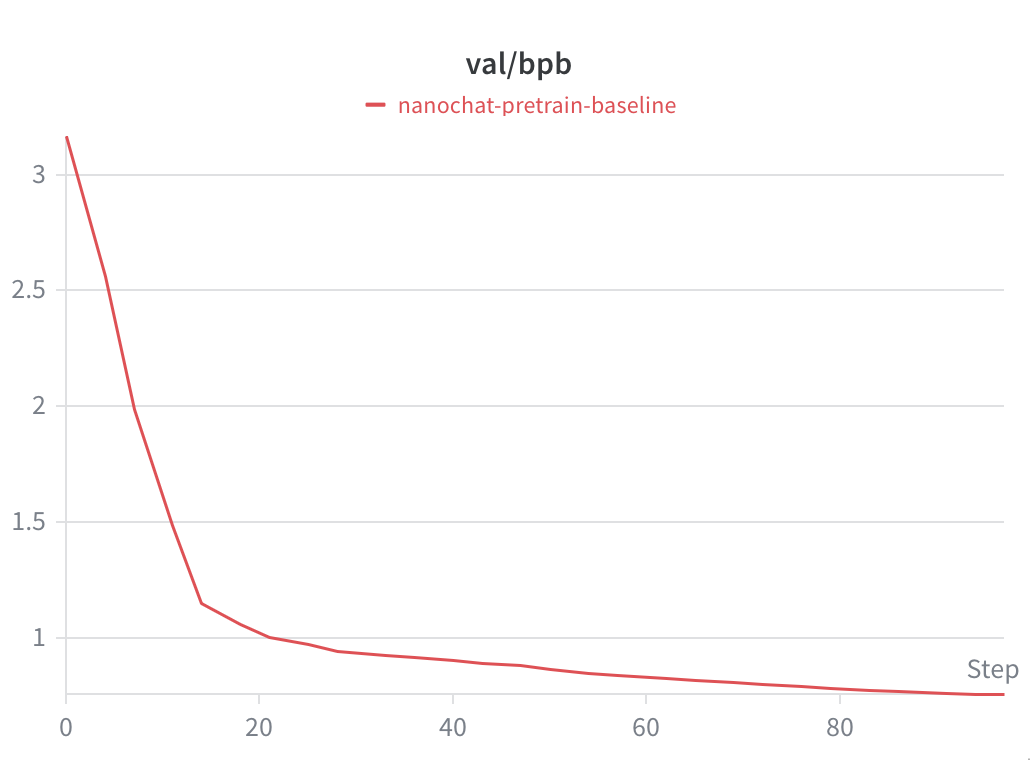
\includegraphics[width=\textwidth]{./images/section2_wandb_pretrain_val_bpb.png}
\end{minipage}\hfill
\begin{minipage}{0.49\textwidth}
    \centering
    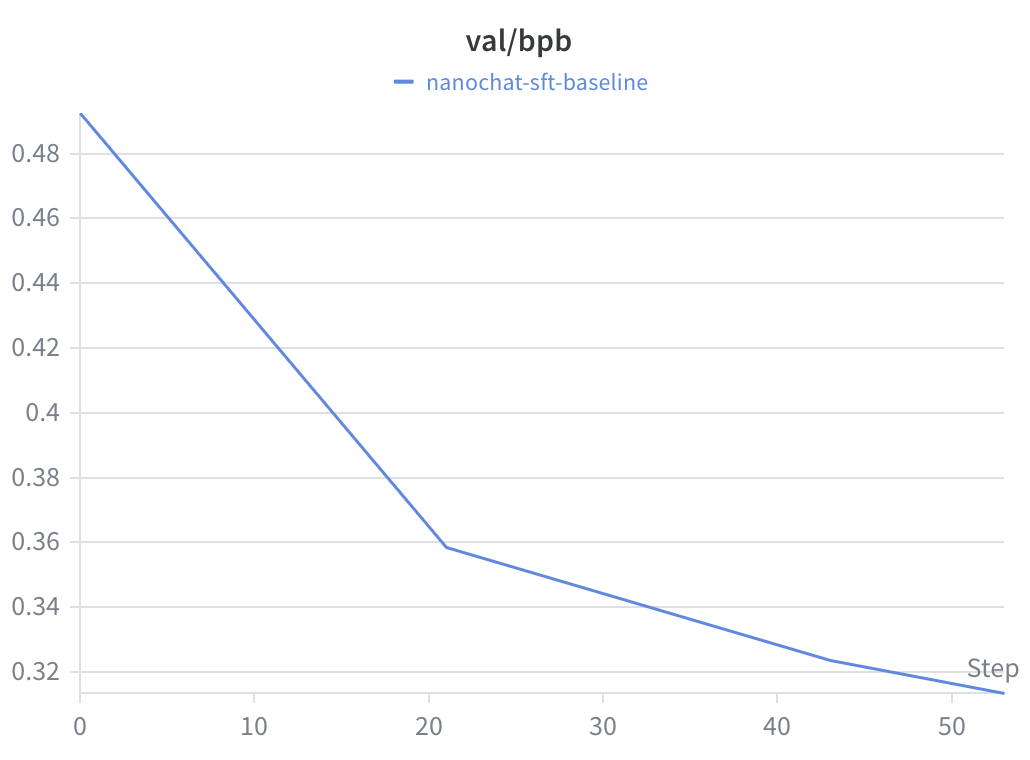
\includegraphics[width=\textwidth]{./images/section2_wandb_sft_val_bpb.png}
\end{minipage}
\caption{Validation BPB curves from Weights \& Biases for the pretraining run (left) and the baseline SFT run (right). The pretraining run reduces held-out loss rapidly at the beginning and then more gradually, while the baseline SFT run continues to push validation BPB downward over its 483-step budget. These optimization curves complement Table~\ref{tab:pretrain-vs-sft} and Figure~\ref{fig:pretrain-vs-baseline-bars}: the W\&B plots show how training progresses, while the final-metric comparison shows how much downstream chat-task performance improves after SFT.}
\label{fig:wandb-pretrain-vs-sft-valbpb}
\end{figure}

The SpellingBee jump is especially dramatic: the pretrained checkpoint scored 0.0000 on that task, while the baseline SFT model reached 1.0000. This is consistent with the composition of the default SFT mixture, which explicitly includes \texttt{SimpleSpelling} and \texttt{SpellingBee} supervision. The pretrained model's base-eval report also helps explain why SFT was necessary: while it achieved a non-trivial CORE score, its qualitative samples remained repetitive and unstable, e.g.\ repeatedly continuing ``\textit{The capital of France is Paris}'' or producing incoherent unconditioned paragraphs. In other words, pretraining produced a competent base language model, but SFT was required to convert that competence into more useful assistant-style behavior.\\

In Figure~\ref{fig:pretrain-vs-baseline-bars}, the six task-specific bars are raw accuracies, whereas ChatCORE is a normalized aggregate score rather than a percentage; accordingly, the vertical axis should be interpreted as \emph{accuracy or normalized score}, not accuracy alone.

\begin{minipage}{1.0\textwidth}
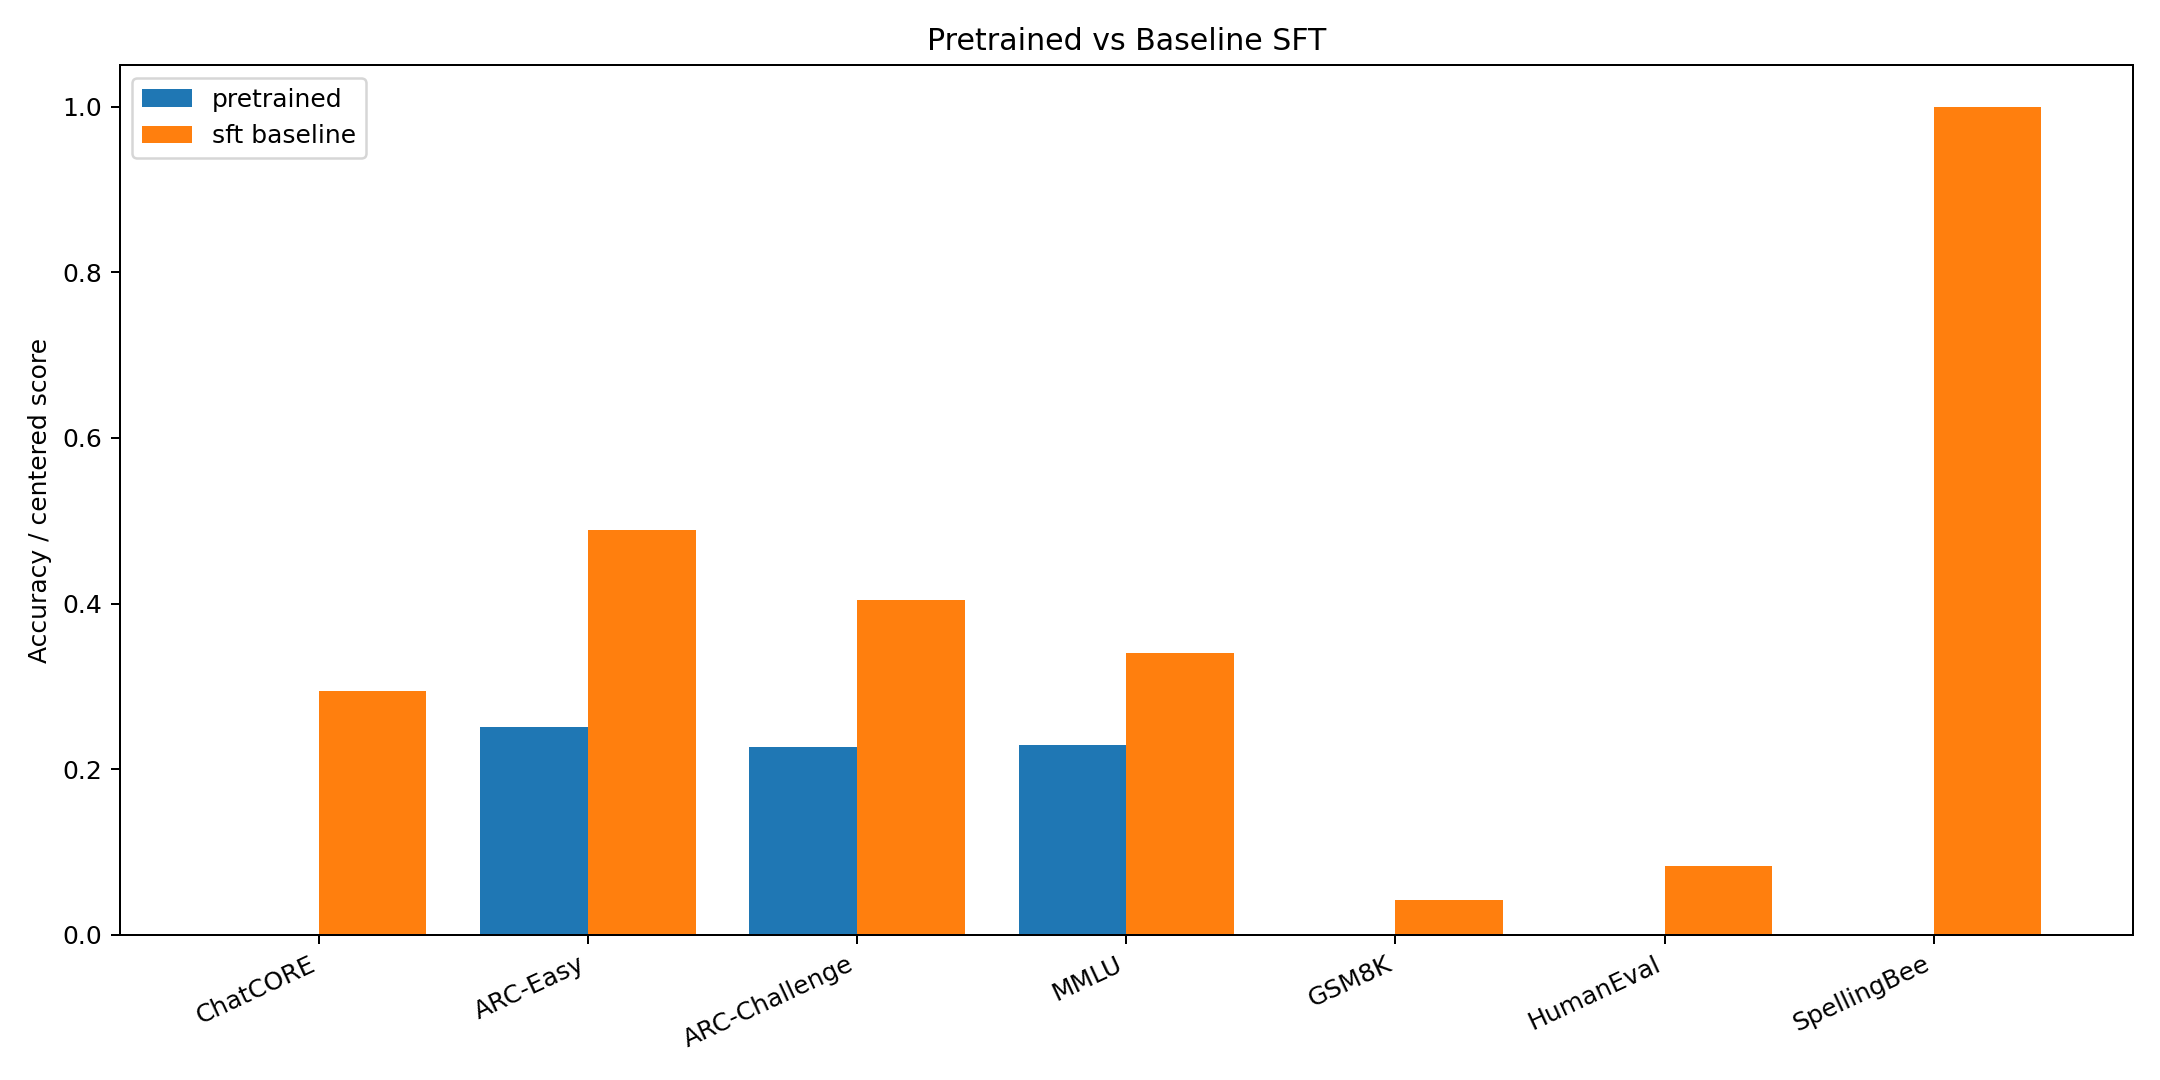
\includegraphics[width=1.0\textwidth]{./images/section2_base_vs_baseline.png}
\label{fig:pretrain-vs-baseline-bars}
\vspace{-0.7cm}
\captionof{figure}{Final-metric comparison of the pretrained checkpoint and the baseline SFT checkpoint on the same chat evaluation suite.}
\end{minipage}

\subsection{Comparison of SFT on Differing Datasets}

\subsubsection{Methodology}
The goal of the added-dataset ablations was not to change the base architecture or optimization parameters, but to test whether augmenting the original SFT data mixture with a small amount of additional high-quality supervised data could improve baseline SFT behavior. To make the comparison fair, both added-dataset runs started from the same pretrained checkpoint as the baseline SFT run, reused the same baseline SFT optimization settings, and were capped at exactly 483 optimizer steps, matching the baseline SFT training budget.

\subsubsection{Dataset Selection}

\begin{enumerate}[label=(\alph*)]
    \item \texttt{ultrachat\_200k} was chosen because it is a large, clean multi-turn conversational dataset and therefore a natural way to test whether increasing the volume of assistant-like dialogue improves general chat behavior beyond the built-in SmolTalk-heavy baseline mixture. It is a good fit for this study because it changes the breadth of conversational supervision without being narrowly optimized for a single benchmark.
    \item \texttt{tulu-3-sft-personas-instruction-following} was chosen because it targets instruction adherence and constraint following more directly than broad chat corpora do. This makes it a better match for the stated goal of making the model more adept at conversation and tasks, rather than simply more verbose or more conversational.
    % \item \texttt{tulu-math} ...
\end{enumerate}

\subsubsection{Quantitative Results}

\begin{table}[ht]
    \centering
    \footnotesize
    \setlength{\tabcolsep}{4pt}
    \begin{tabular}{lcccccccc}
    \toprule
    \textbf{Model} & Val BPB & ChatCORE & ARC-E & ARC-C & MMLU & GSM8K & HumanEval & SpellingBee \\
    \midrule
    \texttt{Baseline SFT} & 0.3135 & 0.2949 & 0.4886 & 0.4044 & 0.3404 & 0.0417 & 0.0833 & 1.0000 \\
    +\ \texttt{tulu-if} & 0.3141 & 0.2886 & 0.4827 & 0.4164 & 0.3371 & 0.0417 & 0.0417 & 1.0000 \\
    % +\ \texttt{tulu-math} & 0. & 0. & 0. & 0. & 0. & 0. & 0. & 0. \\
    +\ \texttt{ultrachat\_200k} & 0.3232 & 0.2608 & 0.4335 & 0.4044 & 0.3358 & 0.0000 & 0.0417 & 0.9583 \\
    \bottomrule
    \end{tabular}
    \caption{Comparison of baseline SFT and added-dataset SFT ablations.}
    \label{tab:sft-ablation-results}
\end{table}

The W\&B trajectory in Figure~\ref{fig:wandb-sft-ablations-chatcore} shows that these differences are not only endpoint effects: the baseline SFT run stays ahead of the two augmented runs for nearly the entire training budget. Looking more closely at the task breakdown, \texttt{tulu-if} slightly improved ARC-Challenge (0.4044 to 0.4164) while leaving GSM8K unchanged, but it lost performance on HumanEval (0.0833 to 0.0417) and slightly reduced ARC-Easy and MMLU. \texttt{ultrachat\_200k} was uniformly weaker than the baseline on ARC-Easy, MMLU, GSM8K, HumanEval, and SpellingBee, while only matching the baseline on ARC-Challenge. The most plausible explanation is budget dilution: because the number of SFT steps was held fixed at 483, the added datasets competed with the baseline mixture for the same optimization budget. Under this constraint, \texttt{tulu-if} appears better aligned with the baseline objective than \texttt{ultrachat\_200k}, while the broader conversational data in Ultrachat likely diluted exposure to the synthetic spelling, math, and evaluation-oriented tasks already present in the baseline mixture. \\

\begin{minipage}{1.0\textwidth}
\centering
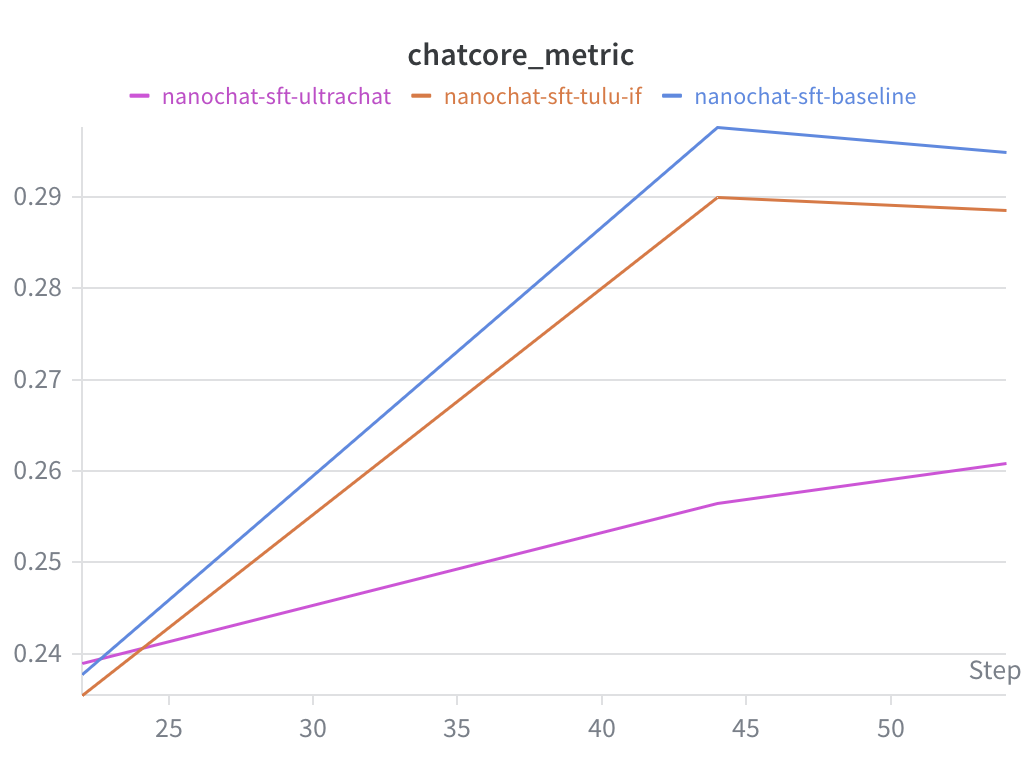
\includegraphics[width=0.75\textwidth]{./images/section2_wandb_chatcore_metric.png}
\label{fig:wandb-sft-ablations-chatcore}
\vspace{-0.5cm}
\captionof{figure}{Weights \& Biases overlay of \texttt{chatcore\_metric} for the baseline SFT run, the SFT run augmented with \texttt{ultrachat\_200k}, and the SFT run augmented with \texttt{tulu-3-sft-personas-instruction-following}. The baseline run remains strongest throughout most of training, \texttt{tulu-if} tracks it closely, and \texttt{ultrachat\_200k} lags consistently. This trajectory-level view is consistent with the final comparison in Figure~\ref{fig:sft-task-breakdown}.}
\end{minipage}

\begin{figure}[t]
\centering
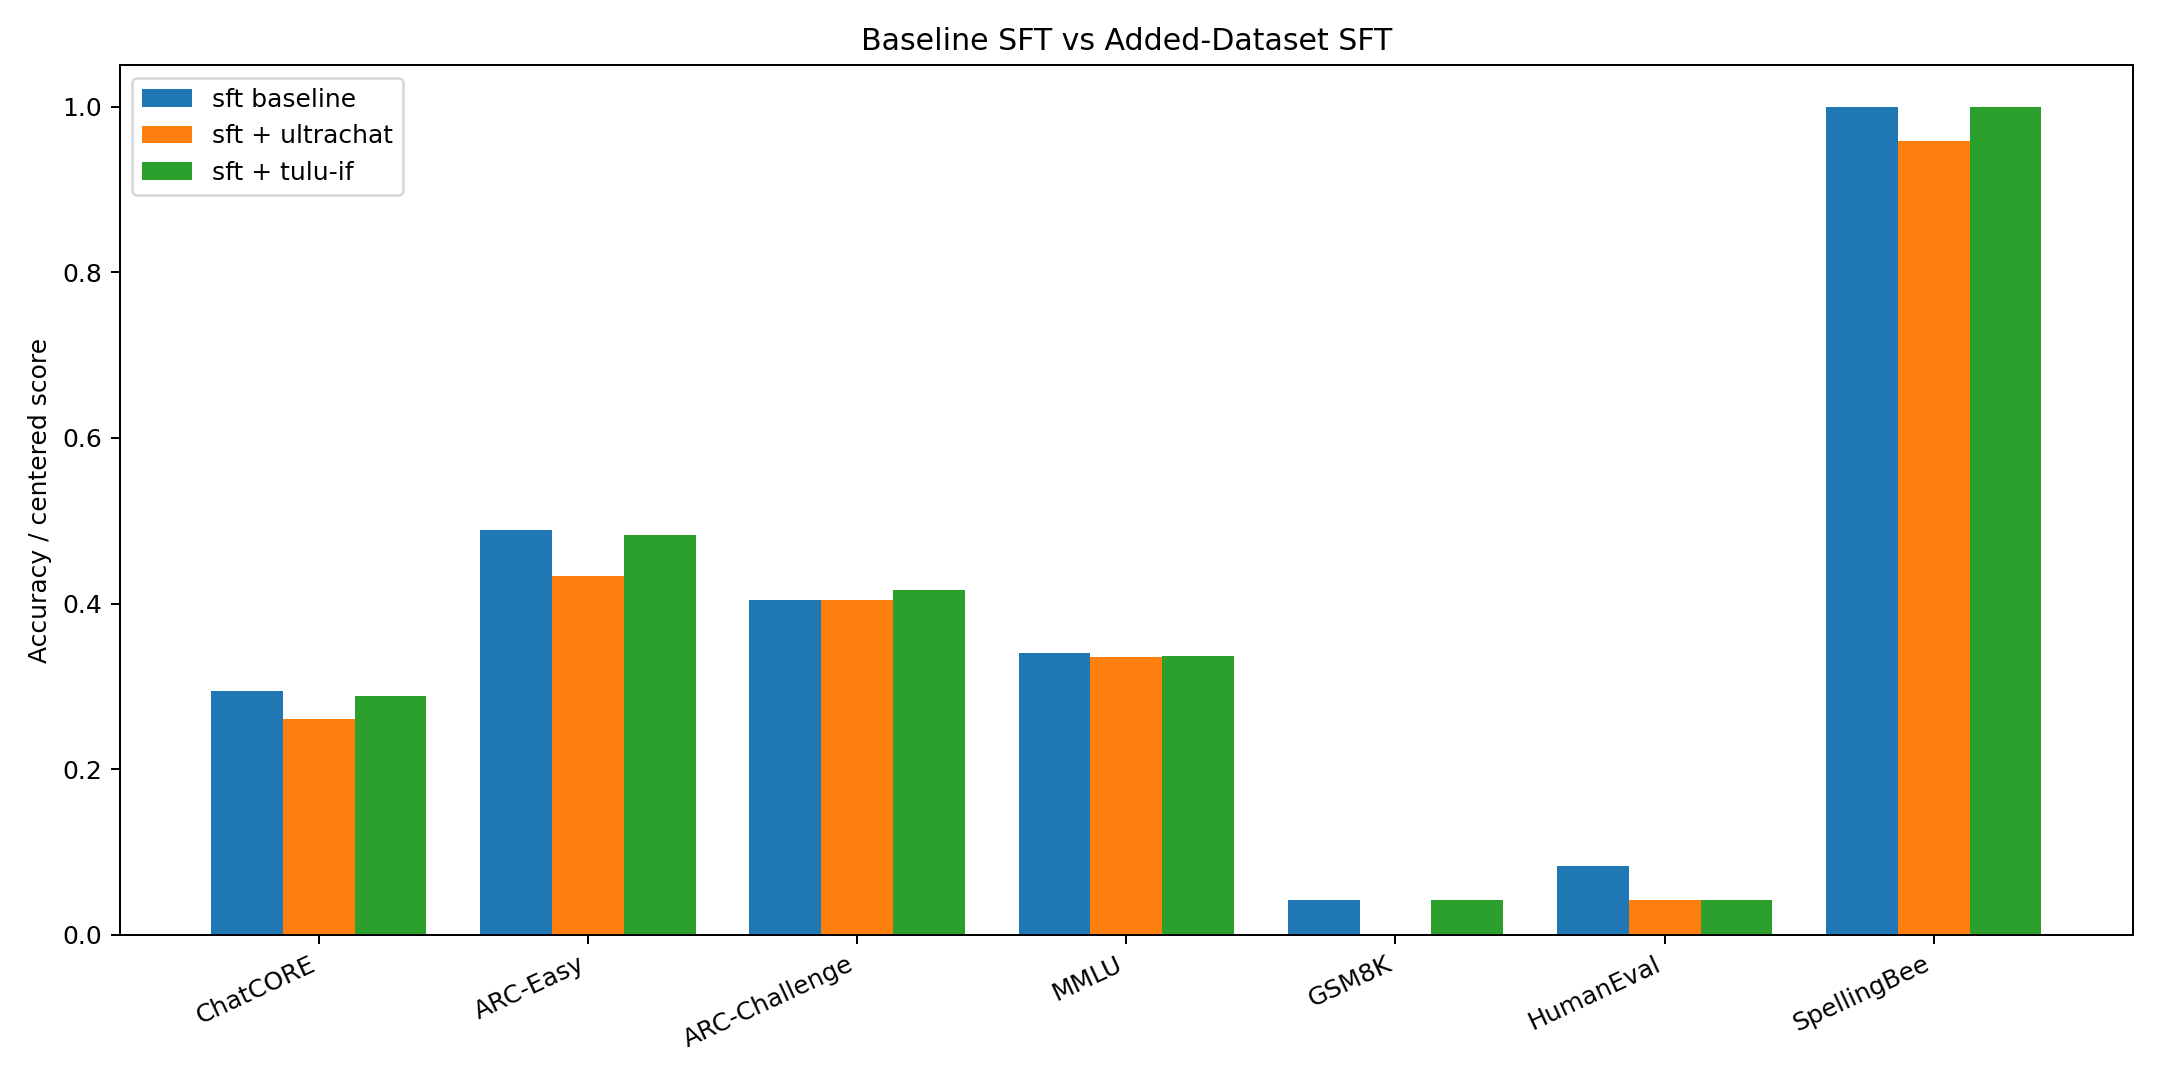
\includegraphics[width=1.0\textwidth]{./images/section2_baseline_vs_augmented.png}
\caption{Final-metric comparison of the baseline SFT run against the two added-dataset SFT ablations.}
\label{fig:sft-task-breakdown}
\end{figure}
\newpage

Overall, the baseline SFT configuration remained the strongest of the three SFT variants we tested. Among the two added datasets, \texttt{tulu-3-sft-personas-instruction-following} was the better fit for the target objective of improving conversational and task-following behavior, but under a fixed 483-step budget it still did not surpass the original baseline recipe. By contrast, \texttt{ultrachat\_200k} appears to have added conversational breadth at the cost of the narrower task competencies measured by the nanochat chat evaluation suite.

% ================================================================================
\section{Replicating Our RL Run With Additional Analysis}
\label{section3}

\subsection{Comparison Between Original and Replicated Runs}

To study the reinforcement-learning phase, we compared three GSM8K RL trajectories: the original \texttt{d20speed} run shown in Karpathy's Discussion \#1 \cite{nanochat-discussion}, our direct attempt to reproduce the default \texttt{chat\_rl.py} configuration on top of our own baseline SFT checkpoint, and a second run in which only the RL learning rates were reduced. In all of our runs, the starting checkpoint was the baseline SFT model \texttt{d24\_sft\_baseline} from Section \ref{section2}. The direct replication attempt used the default \texttt{chat\_rl.py} hyperparameters, whereas the low-learning-rate ablation changed only \texttt{embedding\_lr} from 0.2 to 0.05, \texttt{matrix\_lr} from 0.02 to 0.005, and \texttt{unembedding\_lr} from 0.004 to 0.001; all other RL parameters were left at their script defaults.\\

Figure~\ref{fig:rl-original} shows the original public run reported in Discussion \#1. In that trajectory, the reward curve rises gradually while remaining noisy, \texttt{pass@1} improves from roughly 0.023 to about 0.063, and \texttt{pass@8} increases from about 0.148 to roughly 0.208. This is the behavior we were trying to reproduce: noisy but directionally positive reinforcement learning on GSM8K.\\

\begin{figure}[ht]
\centering
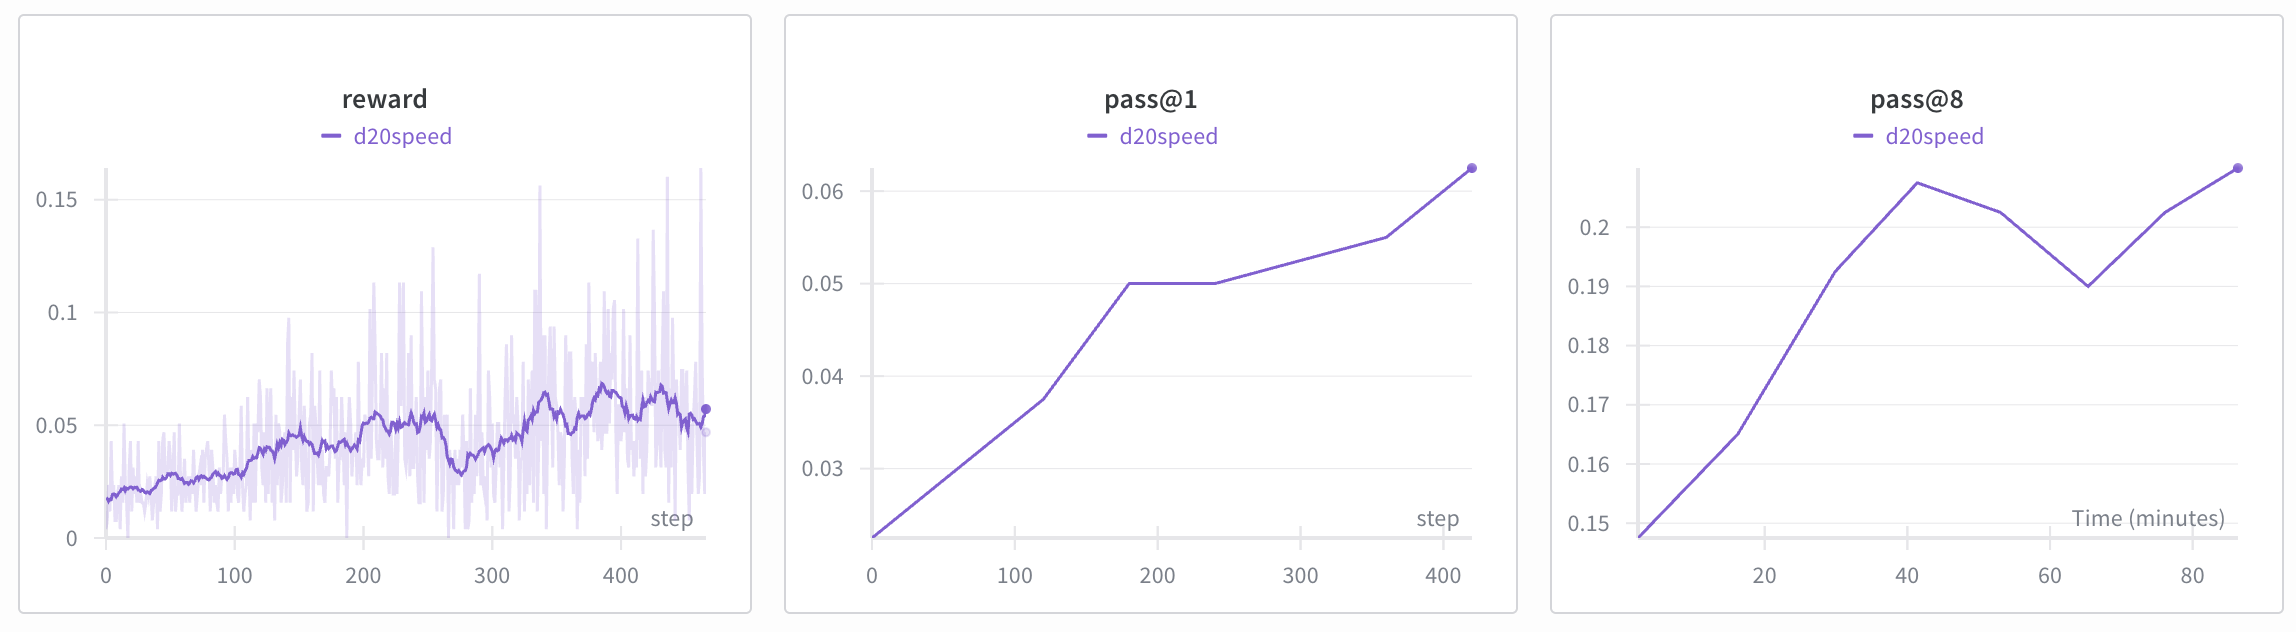
\includegraphics[width=1.0\textwidth]{./images/section3_rl_original_d20speed.png}
\caption{Original nanochat GSM8K RL run from Karpathy's Discussion \#1 (\texttt{d20speed}). The public W\&B plots show a gradually improving reward curve together with rising \texttt{pass@1} and \texttt{pass@8}.}
\label{fig:rl-original}
\end{figure}

Our first attempt to reproduce this behavior with the default RL hyperparameters did not match the original trajectory. As shown in Figure~\ref{fig:rl-ours-default}, the reward rises early but then collapses toward zero, \texttt{pass@1} falls from approximately 0.022 to 0 by around step 240, and \texttt{pass@8} similarly decays from roughly 0.175 to 0. This is not merely slower improvement than the original run; it is a genuine failure mode in which the policy stops finding correct answers altogether.

\begin{figure}[ht]
\centering
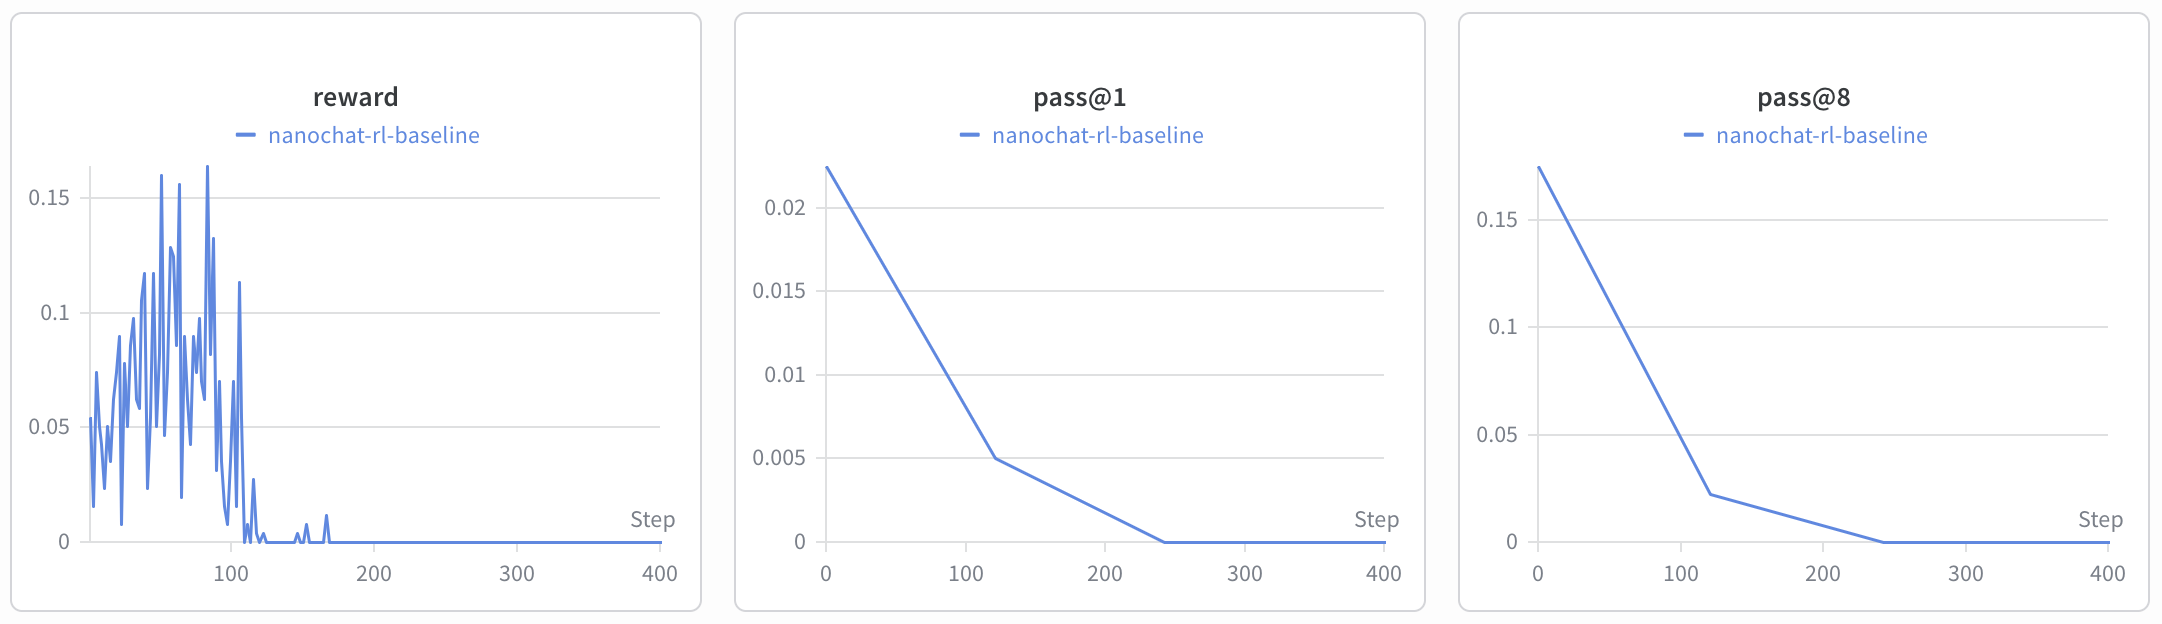
\includegraphics[width=1.0\textwidth]{./images/section3_rl_ours_default.png}
\caption{Our direct replication attempt using the default \texttt{chat\_rl.py} hyperparameters on top of \texttt{d24\_sft\_baseline}. Unlike the original run, reward, \texttt{pass@1}, and \texttt{pass@8} all collapse.}
\label{fig:rl-ours-default}
\end{figure}

The low-learning-rate ablation in Figure~\ref{fig:rl-ours-lowlr} behaved very differently. Here the reward remains noisy but consistently positive throughout training, \texttt{pass@1} rises to roughly 0.097 before ending around 0.087, and \texttt{pass@8} peaks around 0.322 before ending near 0.298. Relative to both the original public run and our own default run, this ablation is substantially more stable and attains markedly better GSM8K evaluation metrics.\\

\begin{figure}[ht]
\centering
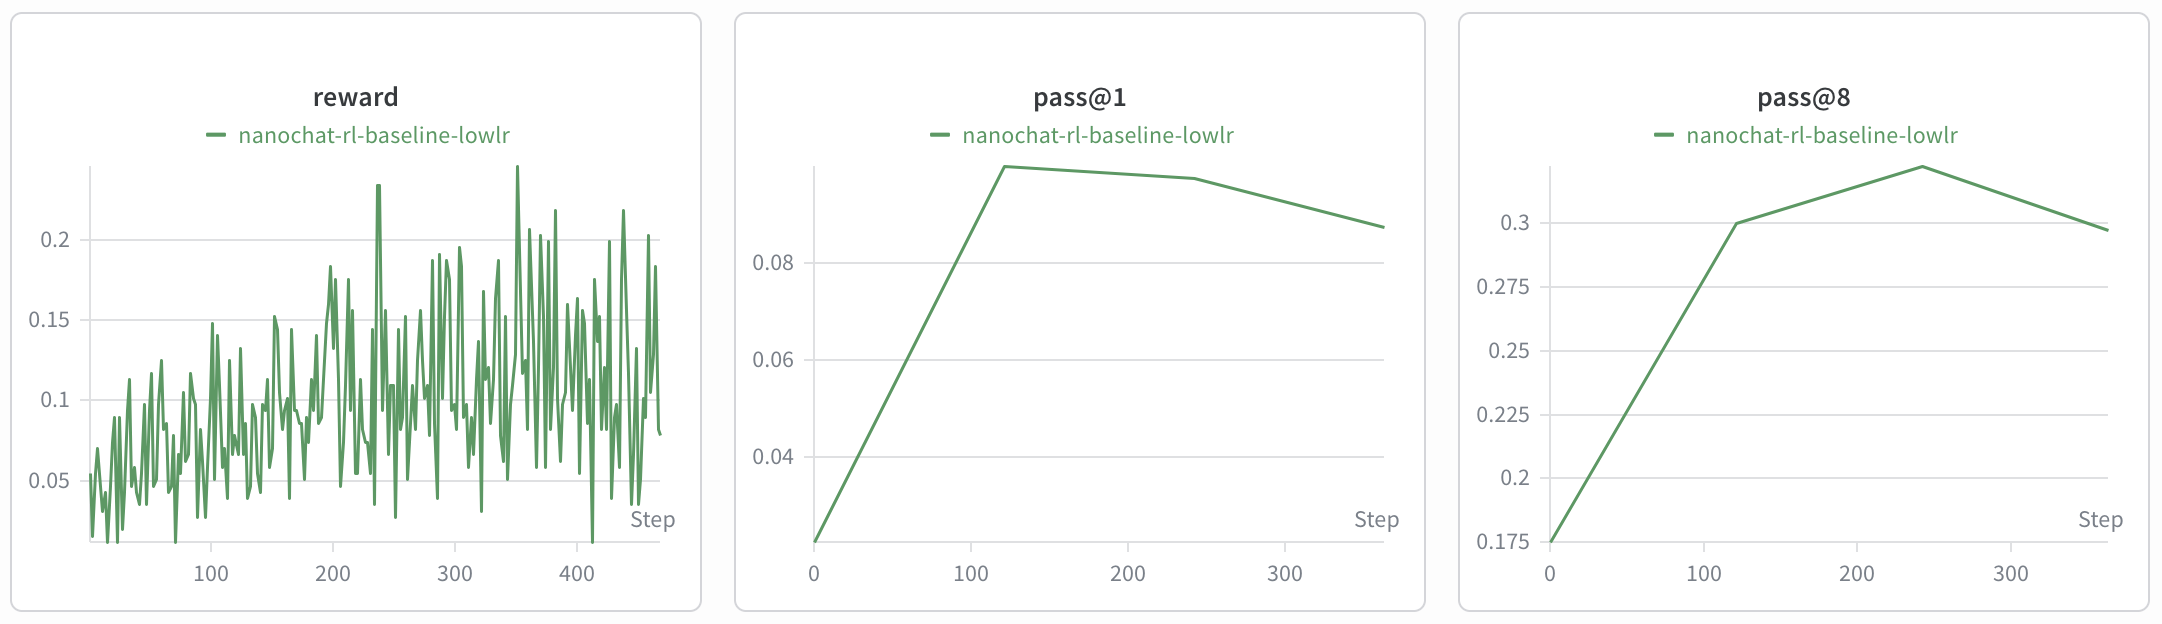
\includegraphics[width=1.0\textwidth]{./images/section3_rl_ours_lowlr.png}
\caption{Our low-learning-rate RL ablation on top of \texttt{d24\_sft\_baseline}. Lowering the RL learning rates prevents the collapse seen in the default run and yields substantially better \texttt{pass@1} and \texttt{pass@8}.}
\label{fig:rl-ours-lowlr}
\end{figure}

The main qualitative conclusion is that the original nanochat RL recipe appears to be highly sensitive to the starting checkpoint and optimization scale. In \texttt{chat\_rl.py}, GSM8K reward is binary, the advantage is simply \texttt{reward - mean(reward)}, and there is no KL regularization, PPO clipping, or trust region. Under this setup, once a run drifts into batches where nearly all samples receive zero reward, the training signal becomes extremely weak and the policy can collapse. That interpretation is consistent with our failed default run.\\

At the same time, the low-learning-rate ablation shows that the discrepancy is not best explained by model depth alone. Karpathy notes in Discussion \#1 that deeper models tended to perform better, and our model is not smaller than the original \texttt{d20speed} model. Instead, our results suggest that the RL stage is unstable under the original default learning rates for our checkpoint, but can be made much more stable by reducing the update magnitude. A second likely factor is that, even when the script is the same, the upstream checkpoint is not identical to the original public run: our pretraining and SFT stages differ from Karpathy's exact speedrun pipeline, and the RL rollouts themselves are stochastic due to sampling at temperature 1.0. Taken together, the most defensible interpretation is that the original RL defaults do not transfer robustly to our model, whereas a simple low-learning-rate ablation does.

\subsection{Error Pattern Review and Exploratory Analysis}

To better understand what the RL runs were actually learning, we performed a post-hoc error analysis on held-out GSM8K examples from the two RL checkpoints: the default RL run (\texttt{rl-default}) and the stabilized low-learning-rate run (\texttt{rl-lowlr}). For each checkpoint, we generated one deterministic answer per problem, recorded whether the answer was correct, and then clustered each example along three axes: (1) \emph{problem cluster} (e.g.\ counting, money/rate, time/rate, geometry, distance, ratio/percent, multi-step), (2) \emph{question complexity} (simple, medium, complex, based on the number of quantities mentioned), and (3) \emph{answer format} (e.g.\ no numeric answer, number without final marker, correct final answer format).\\

The strongest pattern is that the failed default RL run was not primarily making arithmetic mistakes; instead, it was usually failing to produce a usable final answer at all. On our 200-example analysis set, the default run produced \texttt{no\_numeric\_answer} on all 200 examples, while the low-learning-rate run reached 24 correct answers, with the remaining errors distributed across \texttt{wrong\_numeric} (92), \texttt{no\_numeric\_answer} (54), \texttt{magnitude\_error} (22), \texttt{near\_miss} (6), and \texttt{off\_by\_one} (2). This is an important distinction: the low-learning-rate run does not merely improve accuracy, but changes the \emph{type} of failure from ``fails to answer`` to ``attempts an answer but often gets the arithmetic wrong.``\\

\begin{figure}[t]
\centering
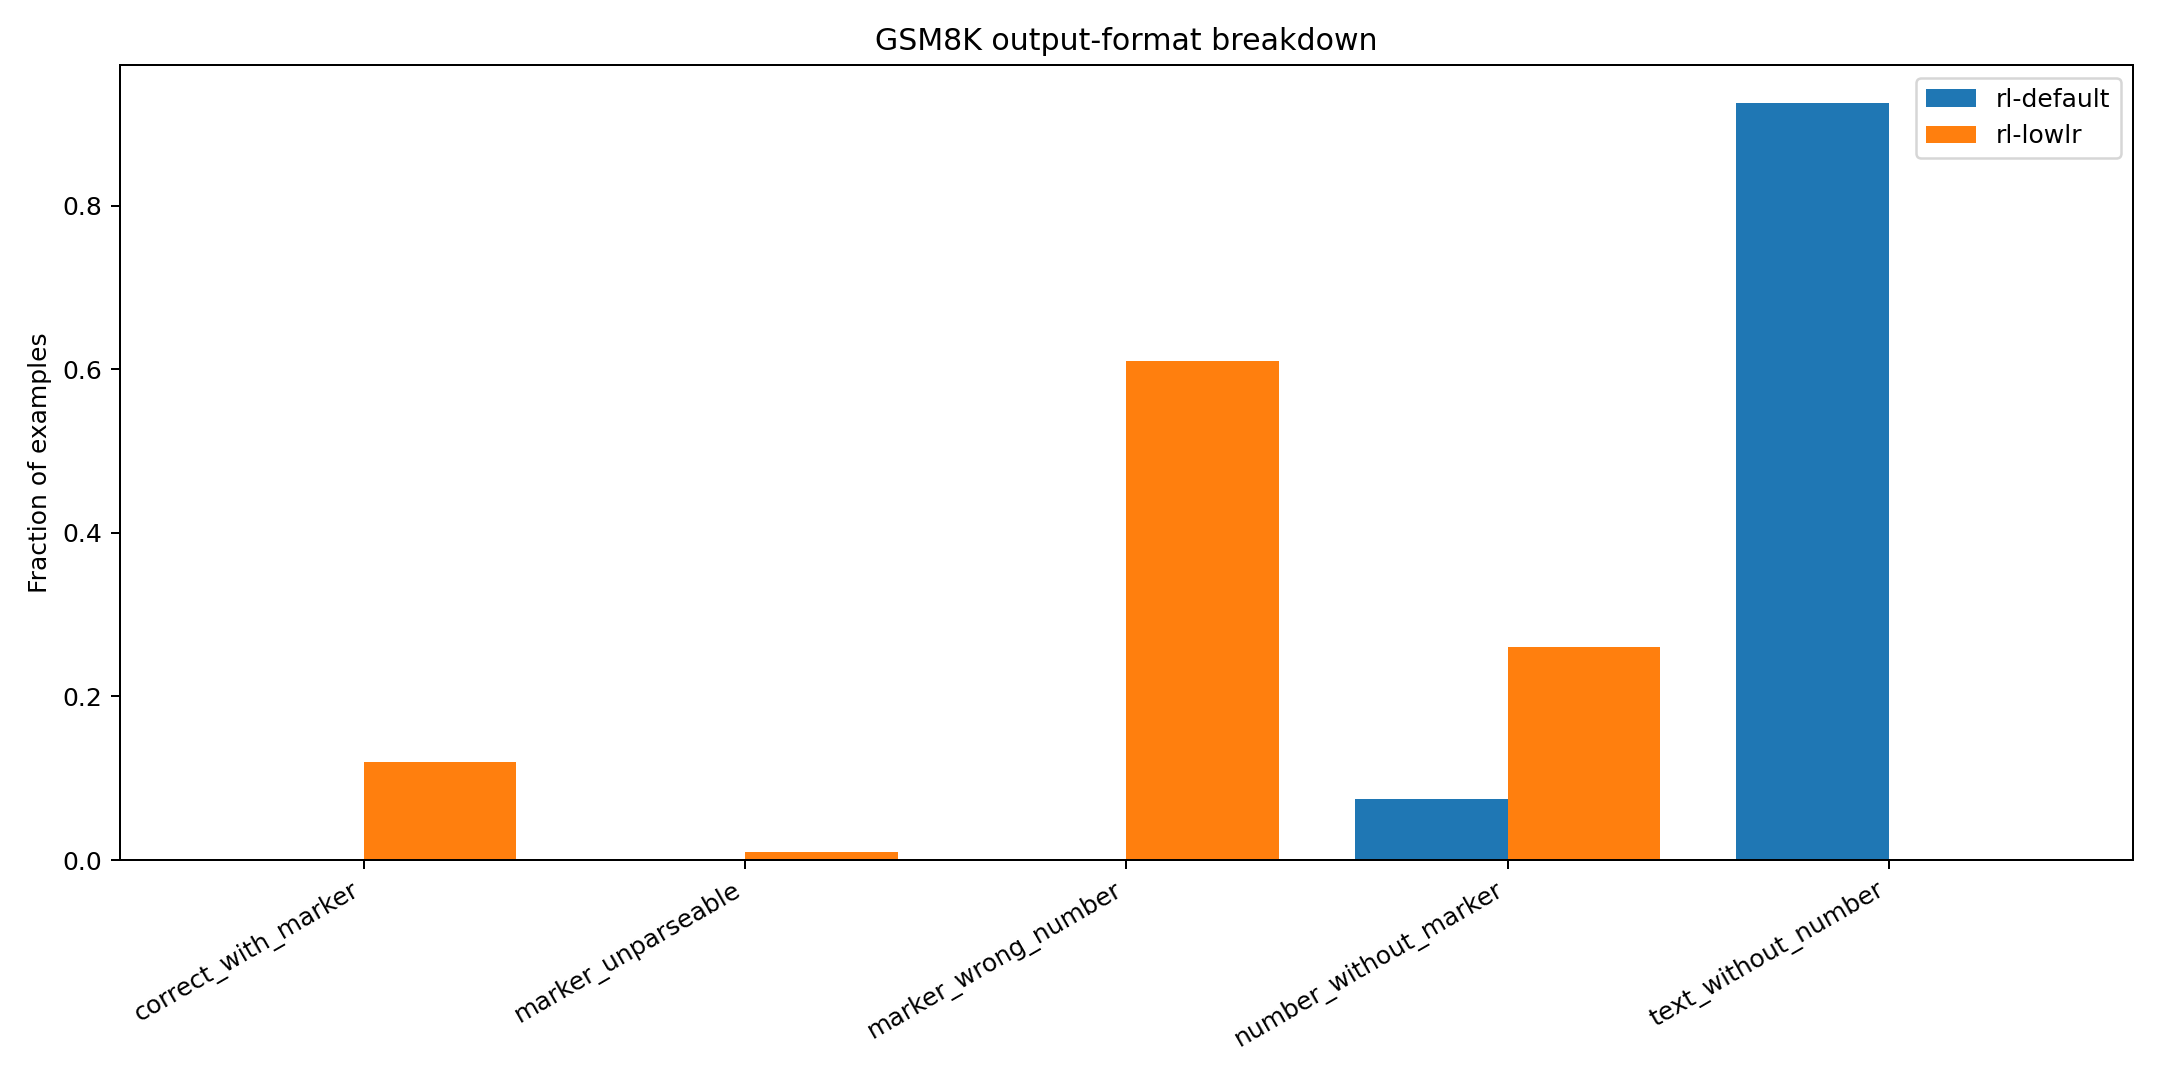
\includegraphics[width=1.0\textwidth]{./images/section3_output_format_breakdown.png}
\caption{Output-format breakdown for the two RL checkpoints. The default RL run is dominated by responses with no parseable numeric answer, whereas the low-learning-rate run shifts much of its mass into numeric outputs, including both correct and incorrect final answers.}
\label{fig:rl-output-format-breakdown}
\end{figure}

Figure~\ref{fig:rl-output-format-breakdown} makes this especially clear. The default RL run is dominated by outputs with text but no parseable number, plus a smaller fraction of answers that contain a number but omit the GSM8K-style final marker. By contrast, the low-learning-rate run produces many more answers in a recognizable problem-solving style, including both \texttt{marker\_wrong\_number} and \texttt{correct\_with\_marker}. In other words, the low-learning-rate run first recovers the ability to produce a structured mathematical answer, and only then begins to improve exact correctness.\\

We also clustered the problems themselves. Figure~\ref{fig:rl-problem-clusters} shows that the low-learning-rate run performs meaningfully better on some categories than others. In our analysis, the best-performing cluster was \texttt{other} (0.5000), followed by \texttt{multi\_step\_other} (0.2000), \texttt{counting} (0.1324), \texttt{time\_rate} (0.1111), and \texttt{money\_rate} (0.0755). However, performance remained at 0 on \texttt{ratio\_percent}, \texttt{distance}, and \texttt{geometry}. This suggests that the stabilized RL run is learning useful behaviour on straightforward counting and rate-style problems, but still struggles badly on more structured quantitative reasoning categories.\\

\begin{figure}[ht]
\centering
\begin{minipage}{1.0\textwidth}
    \centering
    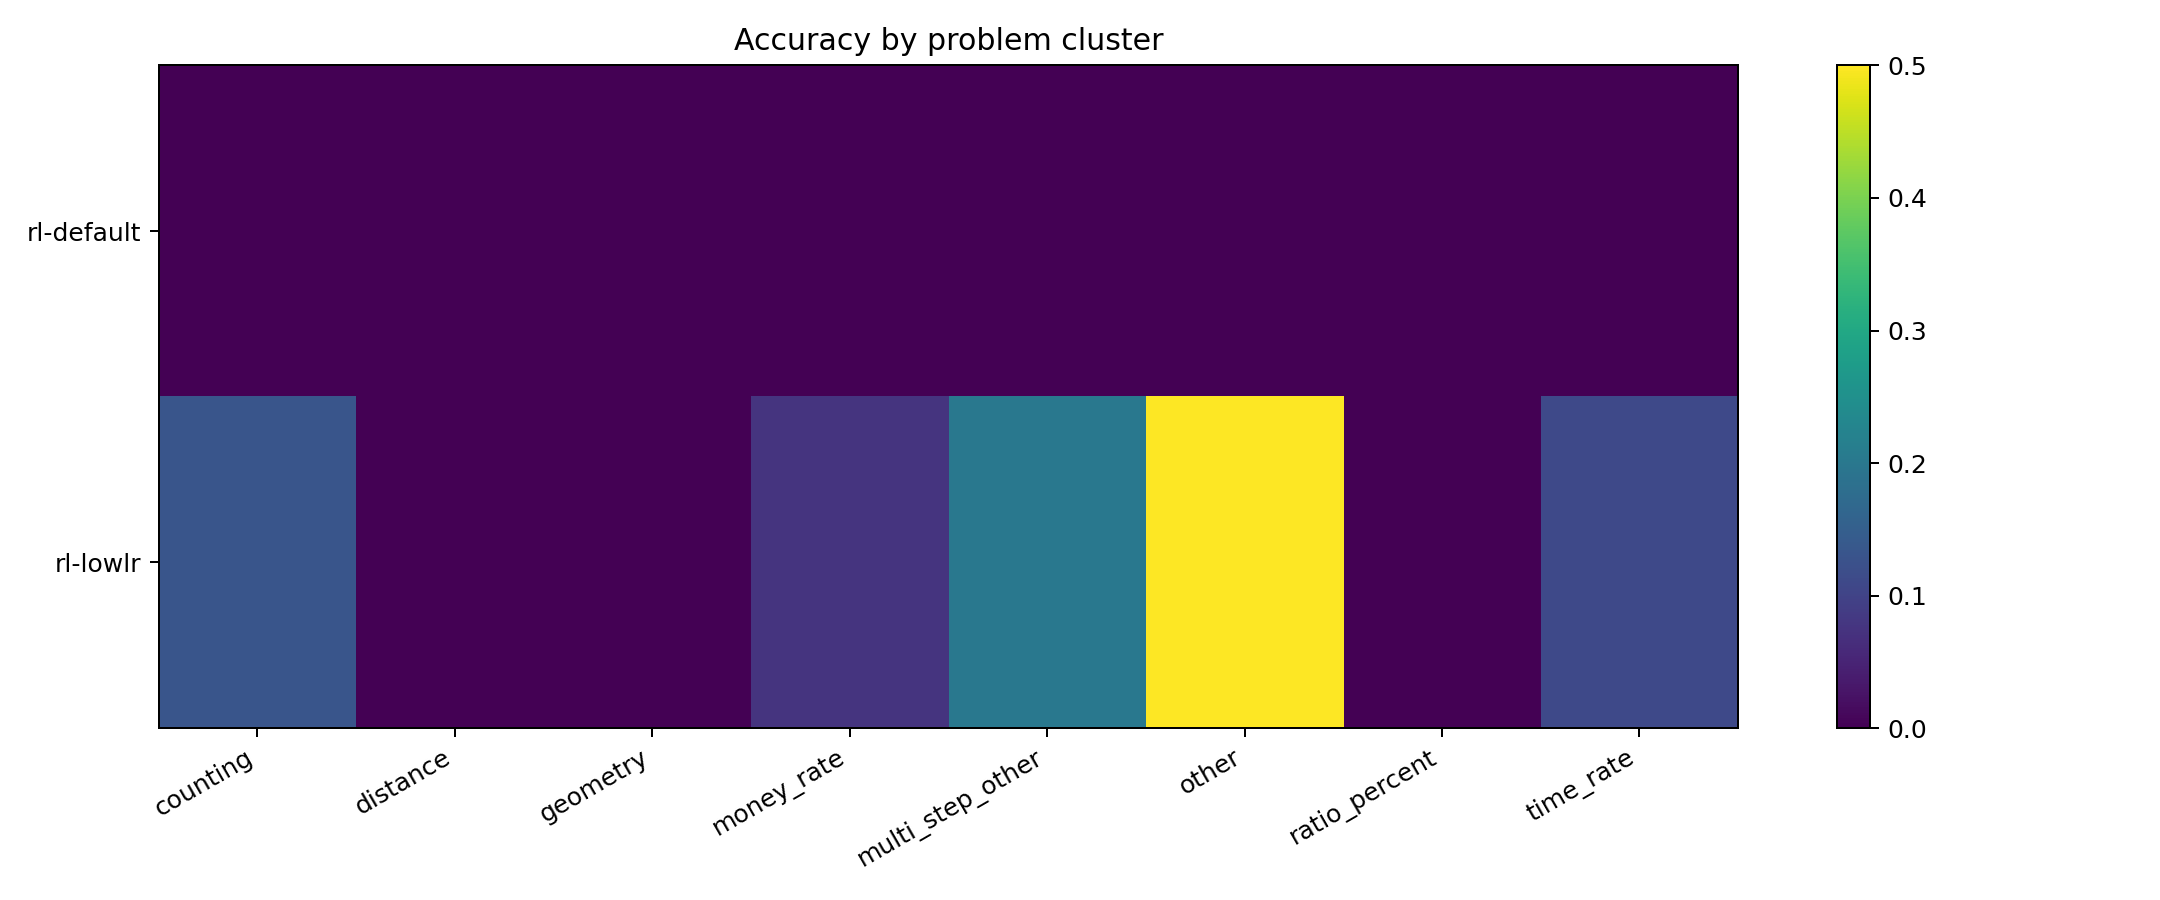
\includegraphics[width=\textwidth]{./images/section3_problem_cluster_heatmap.png}
\end{minipage}\hfill
\begin{minipage}{1.0\textwidth}
    \centering
    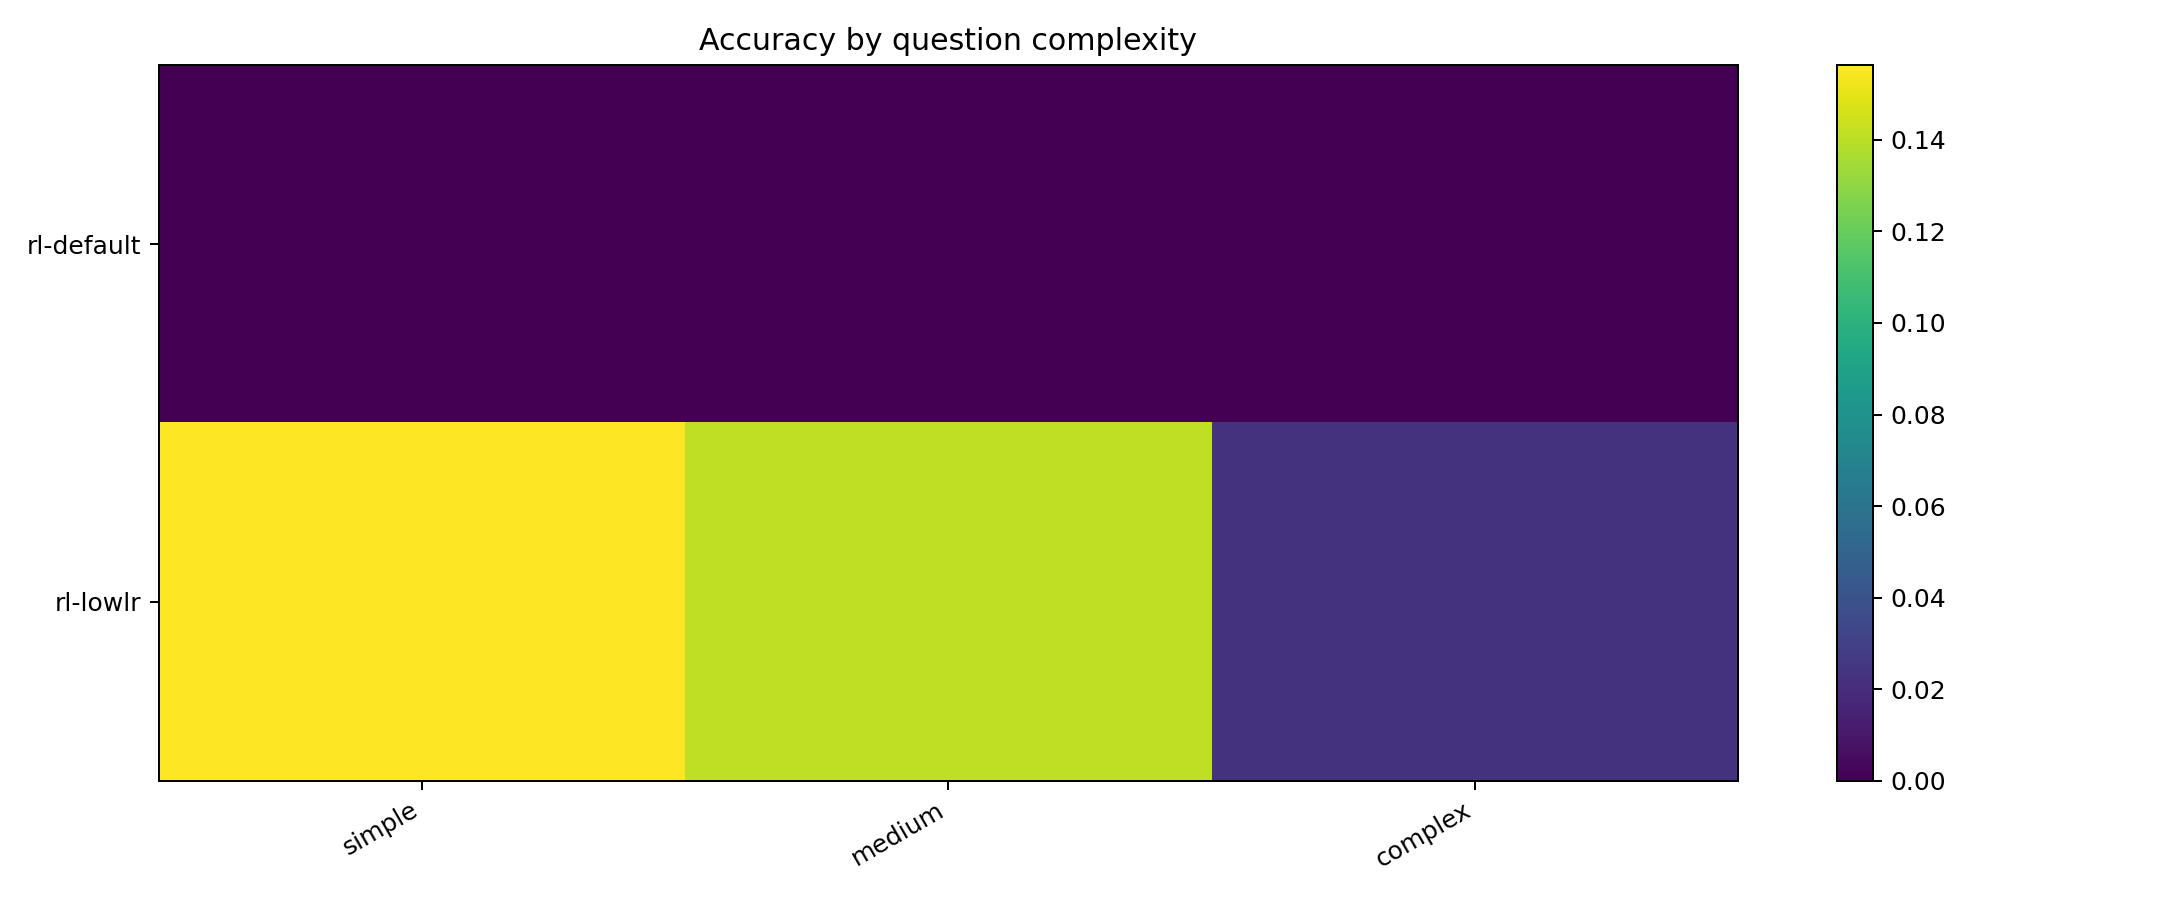
\includegraphics[width=\textwidth]{./images/section3_complexity_heatmap.png}
\end{minipage}
\caption{Exploratory clustering analysis of the RL checkpoints. Left: accuracy by problem cluster. Right: accuracy by question complexity. The low-learning-rate run improves substantially over the default run, but gains are concentrated on simpler categories and collapse on complex problems.}
\label{fig:rl-problem-clusters}
\end{figure}

The complexity analysis tells a similar story. The default run achieves 0 accuracy for simple, medium, and complex questions alike, while the low-learning-rate run reaches 0.1562 on simple problems, 0.1413 on medium problems, and only 0.0227 on complex problems. Thus, the stabilized RL run appears to improve the model's ability to solve relatively direct GSM8K questions, but it does not yet reliably handle longer or more compositionally demanding reasoning chains.\\

Overall, the most important qualitative insight is that the main weakness of the default RL run is \emph{answer production and formatting}, not just mathematical correctness. The low-learning-rate run partially fixes this by producing more worked solutions and more parseable final answers, but many of those answers are still numerically wrong. This pattern strongly suggests that a richer reward system should not rely only on sparse binary correctness, but should separately account for whether the model (1) produces a non-empty response, (2) emits a final numeric answer in the expected format, and (3) computes the correct final result. These observations directly motivate the more complex reward systems proposed in the next section.


% ================================================================================

\section{Introducing a More Complex Reward System}

The error analysis in the previous section showed that the original GSM8K binary reward was too sparse for our model. The dominant failure mode of the original RL run was not merely incorrect arithmetic, but failure to produce a parseable final answer at all: most completions contained text without a usable number, and the baseline checkpoint achieved 0 accuracy on the 200-example post-hoc GSM8K analysis. This suggested that answer production, answer formatting, and exact correctness should be treated as partially separable behaviours rather than collapsed into a single binary reward.\\

To address this, we implemented three new RL environments that preserve the GSM8K task but replace the original binary reward with shaped reward systems. The original binary-reward RL run from the previous section is used here as the primary baseline environment, and the stabilized low-learning-rate RL run from Section \ref{section3} is used as a second, stronger baseline for judging whether the new reward systems improve on a non-collapsed RL policy. The new runs were trained separately from the same SFT checkpoint, using the same rollout, sampling, and evaluation configuration as the RL setup in Section \ref{section3}, with the stabilized low-learning-rate setting retained so that the primary experimental variable is the reward definition itself rather than RL collapse.

\subsection{Reward Environments}

We tested three additional rewards beyond the original binary reward. In the reward definitions below, $r_{\text{nonempty}}$ indicates that the model produced a non-empty completion, $r_{\text{number}}$ indicates that the completion contains a parseable numeric candidate, $r_{\text{marker}}$ indicates that the completion contains a valid GSM8K-style final-answer marker, $r_{\text{worked}}$ indicates that the completion contains a worked-solution trace, $r_{\text{near}}$ indicates that the final answer is numerically close to the gold answer under a relaxed criterion, and $r_{\text{exact}}$ indicates exact answer correctness.

\begin{table}[ht]
\centering
\footnotesize
\begin{tabular}{p{0.15\textwidth} p{0.8\textwidth}}
\hline
\textbf{Environment} & \textbf{Reward definition} \\
\hline
Baseline & $r = \mathbbm{1}[\text{exact final answer}]$ \\
Format & $r = 0.05 r_{\text{nonempty}} + 0.15 r_{\text{number}} + 0.20 r_{\text{marker}} + 0.60 r_{\text{exact}}$ \\
Accuracy & $r = 0.05 r_{\text{nonempty}} + 0.10 r_{\text{number}} + 0.15 r_{\text{marker}} + 0.20 r_{\text{worked}} + 0.20 r_{\text{near}} + 0.30 r_{\text{exact}}$ \\
Combined & $r = 0.05 r_{\text{nonempty}} + 0.10 r_{\text{number}} + 0.15 r_{\text{marker}} + 0.15 r_{\text{worked}} + 0.15 r_{\text{near}} + 0.40 r_{\text{exact}}$ \\
\hline
\end{tabular}
\caption{Reward environments used for the GSM8K RL ablation study.}
\label{tab:reward-systems}
\end{table}

The motivation behind these designs follows directly from Section \ref{section3}. The format-aware reward was intended to reduce the dominant \texttt{text\_without\_number} and \texttt{no\_numeric\_answer} failures by rewarding non-empty answers, numeric content, and valid GSM8K final-answer formatting. The accuracy-shaped reward goes further by also rewarding worked-solution structure and near-miss answers, with the goal of distinguishing completely uninformative failures from partially correct reasoning traces. The combined reward keeps both classes of shaping terms while assigning the largest weight to exact correctness.

\subsection{Quantitative Comparison to the Original RL Run}

Table~\ref{tab:reward-results-summary} summarizes the main results. All three additional reward systems substantially outperform the original RL run from Section \ref{section3}, which remained at 0 accuracy on the 200-example GSM8K analysis set. However, once we compare against the stabilized low-learning-rate run from the previous section, the picture becomes more nuanced. The low-learning-rate baseline reaches 0.1200 accuracy, so only the accuracy-shaped reward clearly exceeds it, reaching 0.1400. The format-aware reward reaches 0.1150, slightly below the low-learning-rate baseline, while the combined reward reaches 0.1000. Thus, all three reward designs successfully improve on the original binary reward, but only the accuracy-shaped environment improves on the stronger low-learning-rate RL baseline in terms of final exact accuracy.

\begin{table}[ht]
\centering
\footnotesize
\setlength{\tabcolsep}{3.5pt}
\begin{tabular}{lcccccc}
\hline
\textbf{Run} & \textbf{Accuracy} & \textbf{Simple} & \textbf{Medium} & \textbf{Complex} & \textbf{Correct} & \textbf{Dominant failure} \\
\hline
Original RL & 0.0000 & 0.0000 & 0.0000 & 0.0000 & 0.0000 & non numeric \\
Low-LR RL & 0.1200 & 0.1562 & 0.1413 & 0.0227 & 0.1200 & wrong number / no marker \\
Format-aware & 0.1150 & 0.1562 & 0.1413 & 0.0000 & 0.1150 & wrong number \\
Accuracy-shaped & 0.1400 & 0.1875 & 0.1739 & 0.0000 & 0.1400 & wrong number \\
Combined & 0.1000 & 0.1406 & 0.1196 & 0.0000 & 0.1000 & wrong number \\
\hline
\end{tabular}
\caption{Summary of the GSM8K reward-system results. Accuracy is measured on the 200-example post-hoc analysis set. ``Correct'' denotes the fraction of examples with a correctly formatted and correct final answer under the output-format analysis.}
\label{tab:reward-results-summary}
\end{table}

The training curves collected in Weights \& Biases showed the same general ranking among the three new reward systems. The accuracy-shaped run maintained the highest average reward during training, the combined run finished with the strongest \texttt{pass@1}, and the accuracy-shaped run finished with the strongest \texttt{pass@8}. Taken together with Table~\ref{tab:reward-results-summary}, these trajectories suggest that the shaped rewards improved both training stability and downstream answer quality relative to the original binary reward, even though the best reward for final exact accuracy was not necessarily the same as the best reward for every training-time metric.

\begin{figure}[ht]
\centering
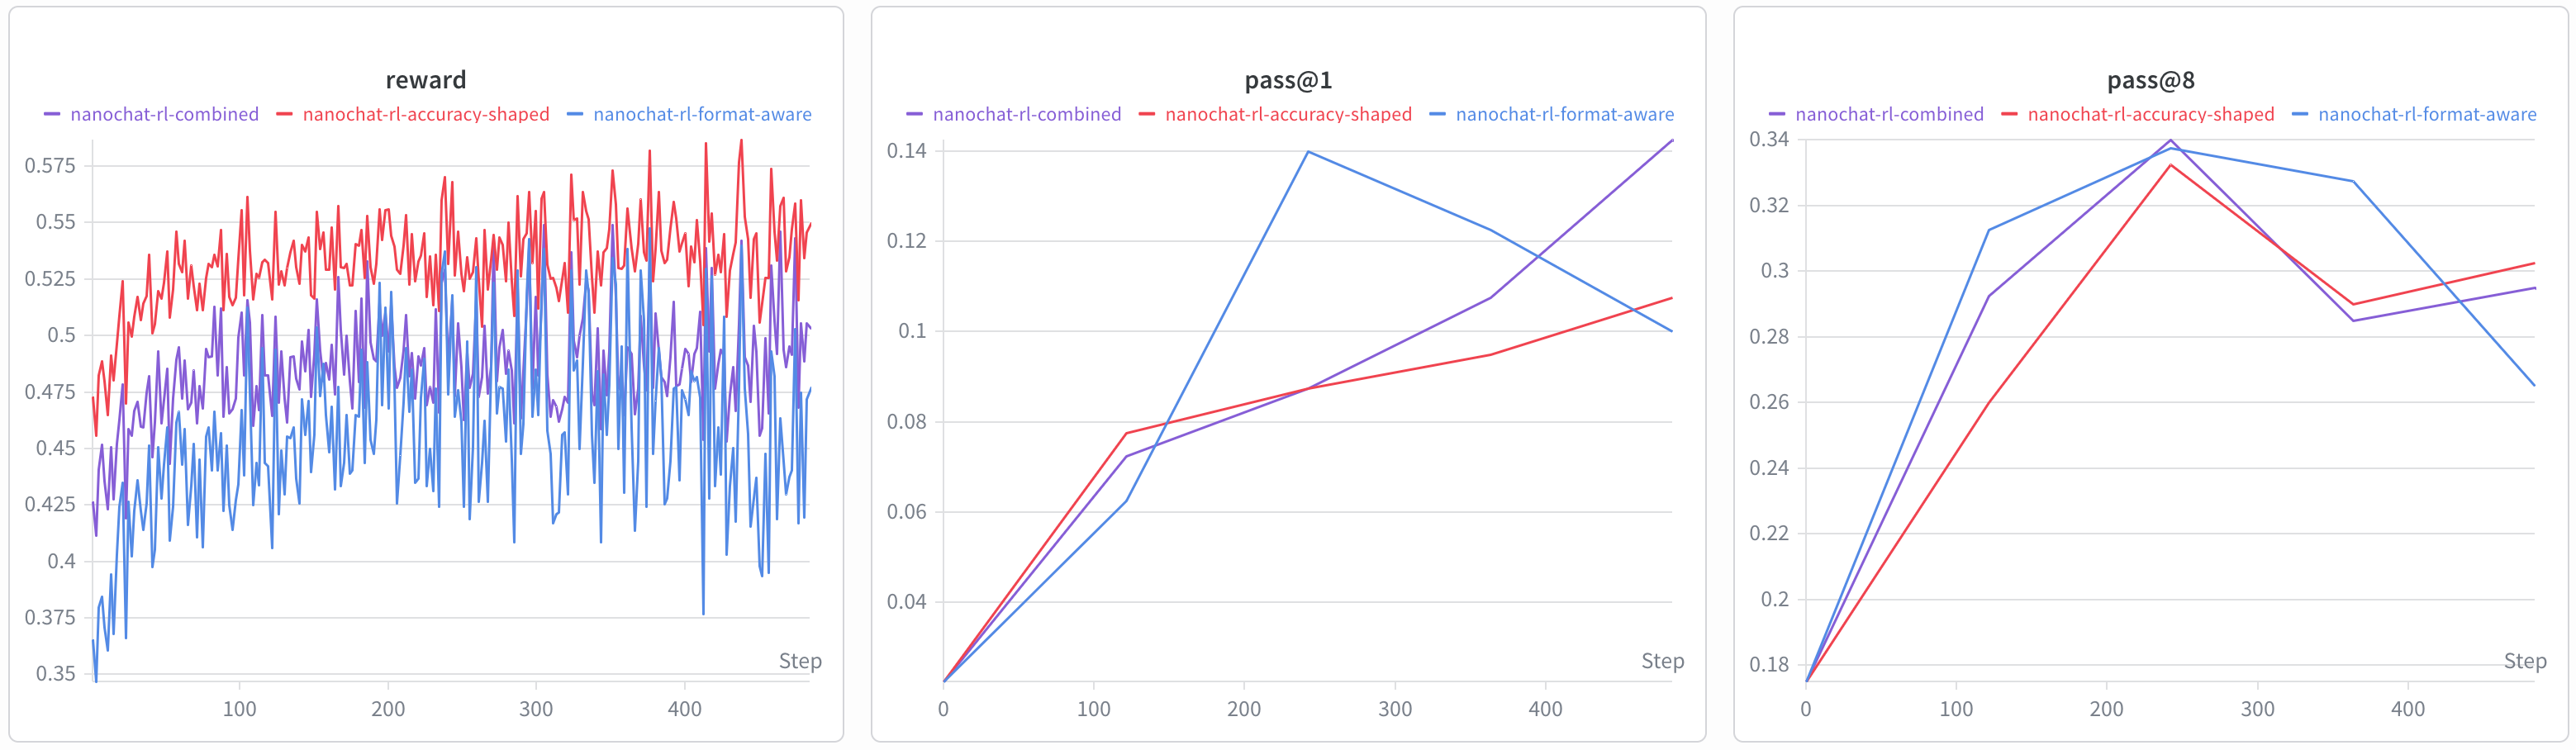
\includegraphics[width=1.0\textwidth]{./images/section4_wandb_new_runs.png}
\caption{Weights \& Biases reward and evaluation curves for the three new reward environments. The accuracy-shaped run maintains the strongest reward signal throughout training and finishes with the strongest \texttt{pass@8}, while the combined reward finishes with the strongest \texttt{pass@1}. The format-aware run improves quickly early on, but does not maintain the same final evaluation strength as the accuracy-shaped reward.}
\label{fig:reward-wandb-new-runs}
\end{figure}

\begin{figure}[ht]
\centering
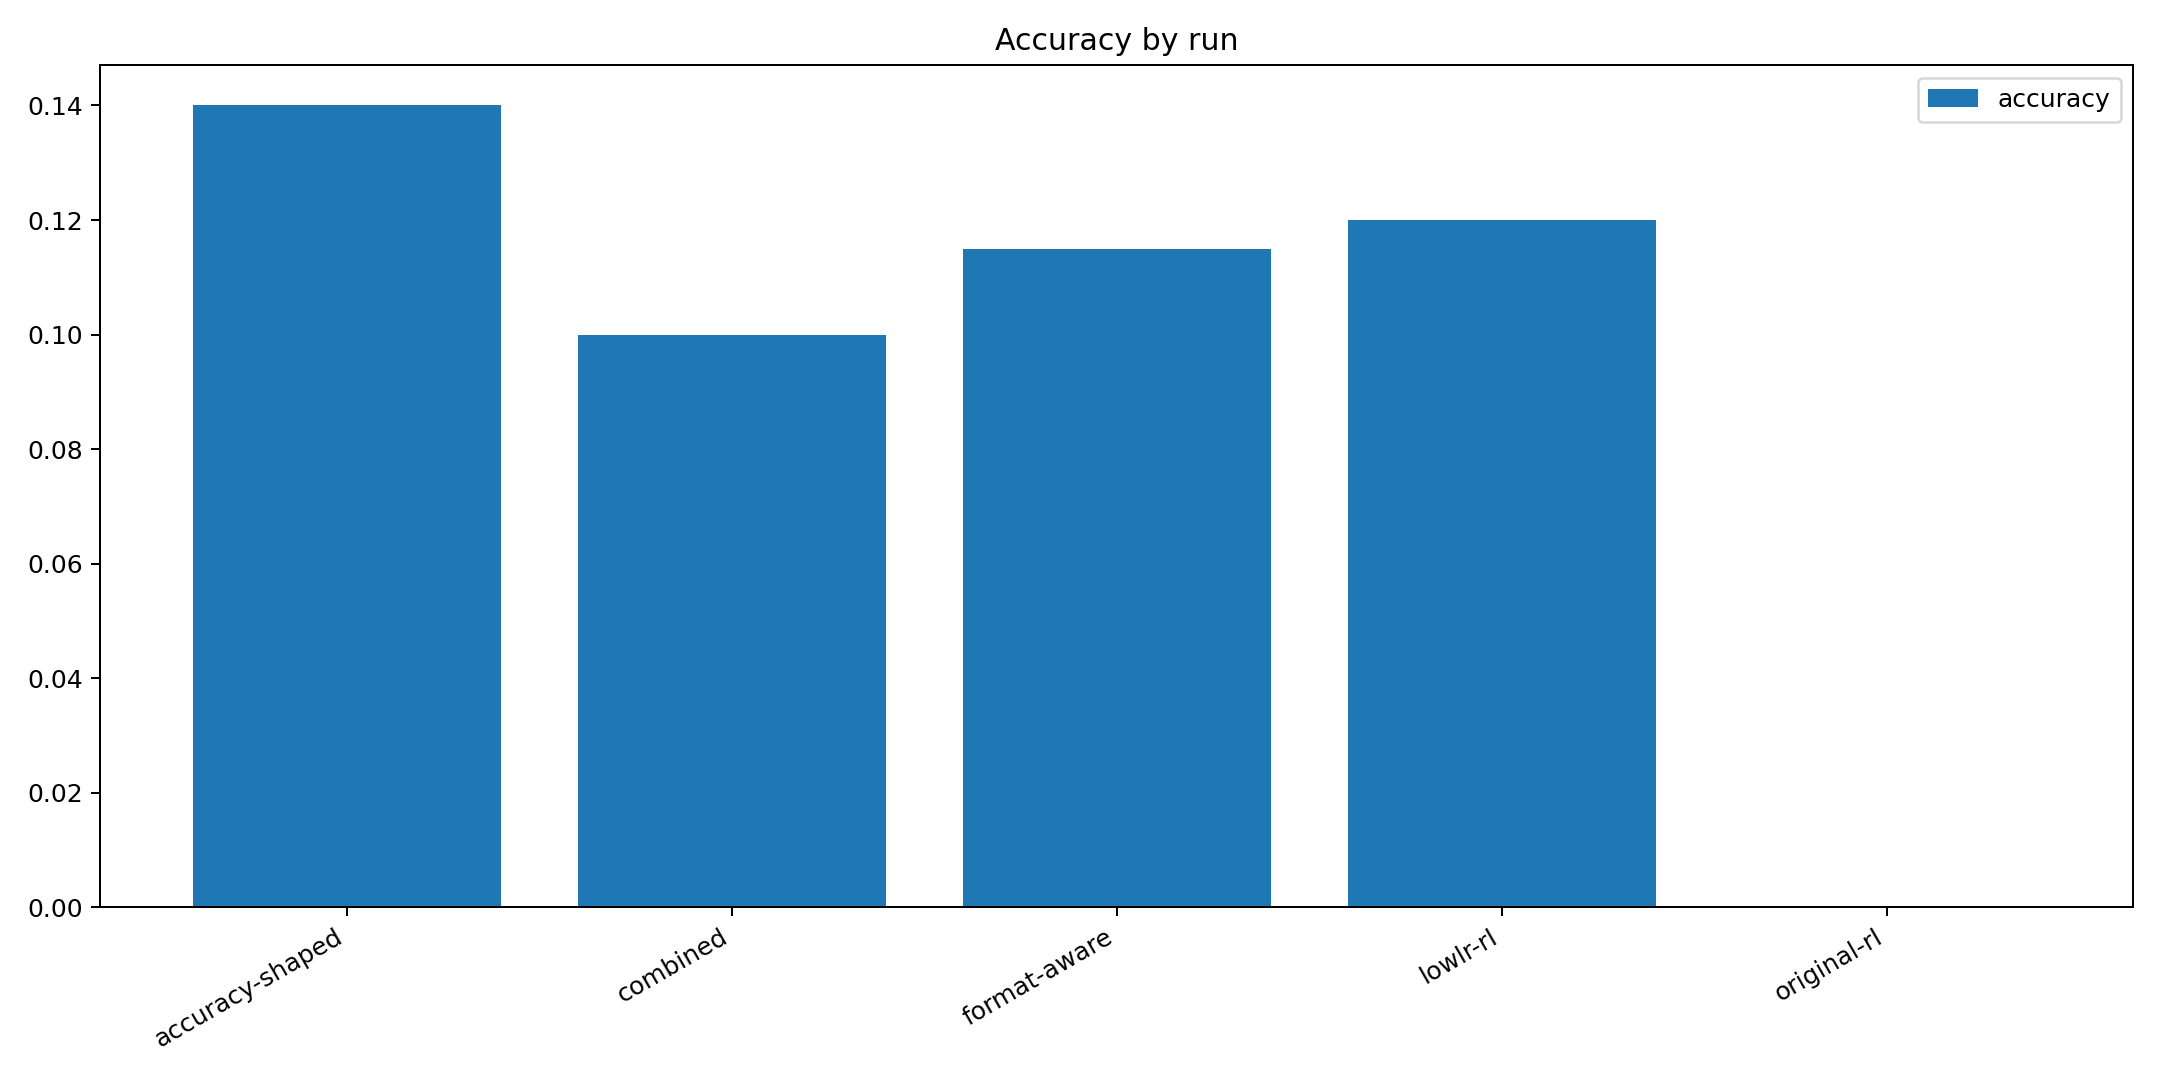
\includegraphics[width=1.0\textwidth]{./images/section4_accuracy.png}
\caption{Overall GSM8K accuracy by run. All three shaped reward systems outperform the original binary-reward RL baseline from Section \ref{section3}; compared to the stabilized low-learning-rate RL run, only the accuracy-shaped reward improves final exact accuracy.}
\label{fig:reward-accuracy}
\end{figure}

\subsection{How the Rewards Changed the Types of Mistakes}

The most important qualitative shift is that the new rewards changed the model's failures from \emph{non-answer failures} into \emph{attempted mathematical answers}. Figure~\ref{fig:reward-output-format} shows this clearly. In the original RL run, 92.5\% of the analysed examples fell into \texttt{text\_without\_number}, and the remaining 7.5\% fell into \texttt{number\_without\_marker}. In other words, the baseline model almost never produced a valid final GSM8K answer at all. The stabilized low-learning-rate run already improved this substantially, shifting failures into 61.0\% \texttt{marker\_wrong\_number}, 26.0\% \texttt{number\_without\_marker}, and 12.0\% \texttt{correct\_with\_marker}.\\

By contrast, the shaped reward systems almost completely eliminated the \\\texttt{text\_without\_number} failure mode and, relative to the low-learning-rate baseline, further reduced incomplete final-answer formatting. The format-aware run shifted 79.5\% of examples into \texttt{marker\_wrong\_number} and 11.5\% into \texttt{correct\_with\_marker}, with only 8.5\% remaining as \texttt{number\_without\_marker}. The accuracy-shaped run improved this further, reaching 14.0\% \texttt{correct\_with\_marker} while reducing \texttt{number\_without\_marker} to 3.0\%. The combined reward still produced structured answers, but underperformed the accuracy-shaped reward with 10.0\% \texttt{correct\_with\_marker}. This shows that the additional rewards did not merely increase accuracy; they changed the \emph{format} and \emph{usability} of the model's answers, and in the case of the accuracy-shaped reward they also improved on the stronger low-learning-rate baseline.\\

\begin{figure}[ht]
\centering
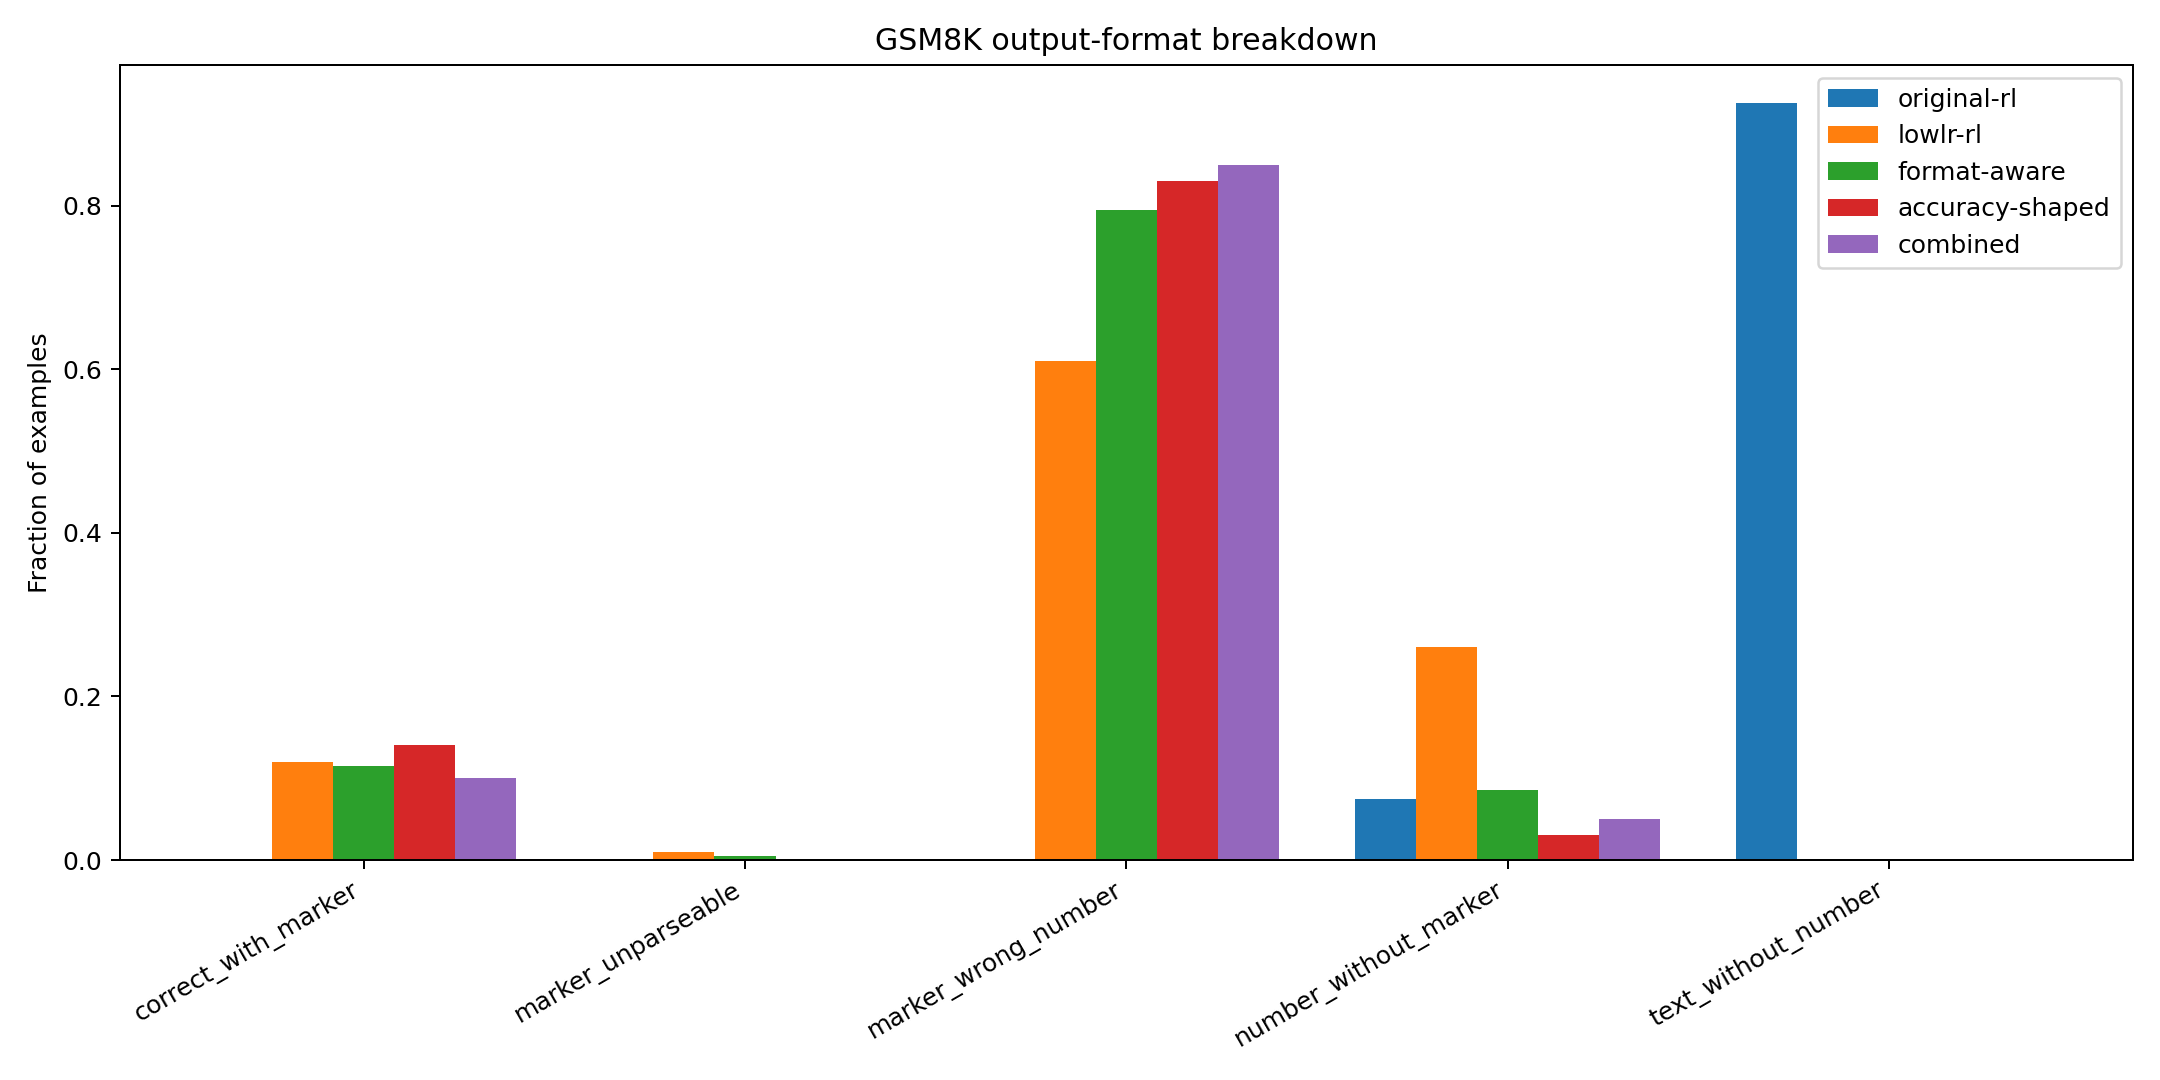
\includegraphics[width=1.0\textwidth]{./images/section4_output_format_breakdown.png}
\caption{Output-format breakdown across the original RL baseline, the low-learning-rate RL baseline, and the three new reward systems. The main effect of reward shaping is to reduce non-answer and no-marker failures further, shifting the model toward correctly formatted final answers even when the arithmetic remains imperfect.}
\label{fig:reward-output-format}
\end{figure}

Figure~\ref{fig:reward-error-types} shows the corresponding change in error types. The original RL run is dominated by \texttt{no\_numeric\_answer}. The low-learning-rate RL run already shifts many failures into \texttt{wrong\_numeric}, \texttt{magnitude\_error}, and a smaller number of correct answers. Once the new rewards are introduced, the dominant failures remain arithmetic rather than formatting failures, but the relative mix changes: the accuracy-shaped run produces the largest number of correct answers (28) and the smallest number of non-numeric failures (6), while the format-aware and combined runs still improve substantially over the original RL baseline but do not exceed the low-learning-rate run as clearly. This is a meaningful improvement: the model is no longer failing at the level of ``produce a usable answer'' but instead at the level of ``perform the right arithmetic.''\\

\begin{figure}[ht]
\centering
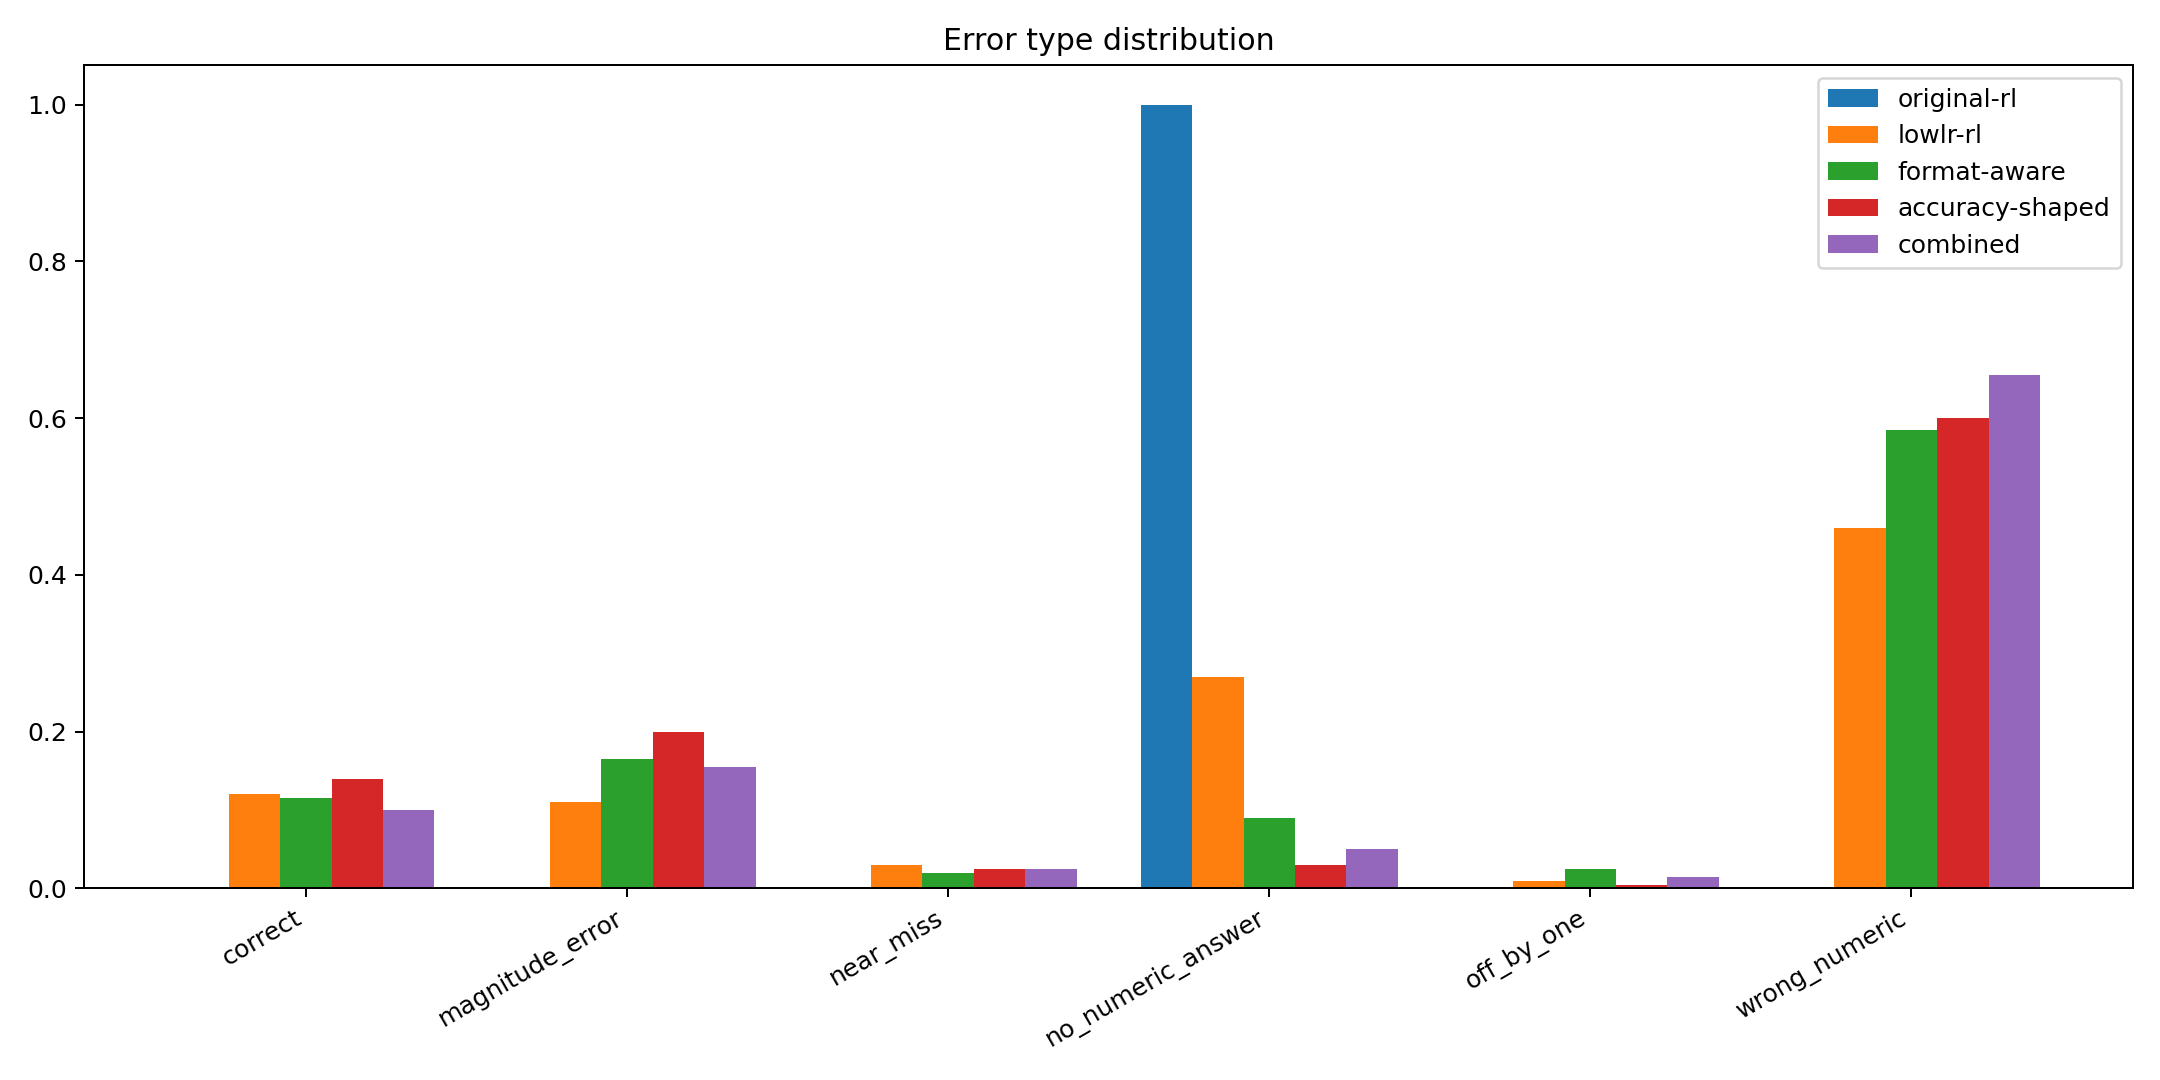
\includegraphics[width=0.9\textwidth]{./images/section4_error_types_by_run.png}
\caption{Distribution of error types for the original RL run, the low-learning-rate RL run, and the three shaped-reward runs. Relative to the low-learning-rate baseline, the accuracy-shaped reward gives the clearest improvement in exact correctness while keeping non-numeric failures low.}
\label{fig:reward-error-types}
\end{figure}

The disagreement examples support this interpretation. For many questions, the original RL baseline produced a blank or unparseable answer, while the low-learning-rate and shaped-reward runs generated a worked solution ending in a numeric result. In several cases, the accuracy-shaped reward solved problems that the low-learning-rate, format-aware, and combined rewards still missed, especially on money/rate or multi-step arithmetic items. For example, on a problem about splitting fundraising revenue across students, the accuracy-shaped run produced the correct answer 6250, while the low-learning-rate run produced 3750, the format-aware run emitted a non-numeric answer, and the combined run produced a large magnitude error. Similarly, on several ratio or multi-step counting problems, the accuracy-shaped run reached the correct answer while the other reward systems still made arithmetic mistakes.

\subsection{Clustering the Remaining Failures}

We also clustered the GSM8K problems by type and by question complexity. The high-level trend is encouraging but incomplete. The shaped rewards improve simple and medium problems substantially, but compared to the low-learning-rate baseline they do not improve every part of the distribution uniformly. Accuracy-shaped again performs best on simple and medium questions, reaching 0.1875 and 0.1739 respectively, while the low-learning-rate run remains the only nonzero run on the complex bucket at 0.0227. Thus, the new rewards improve average accuracy, but they do not yet solve the hardest reasoning cases better than the stabilized low-learning-rate baseline.\\

\begin{figure}[ht]
\centering
\begin{minipage}{1.0\textwidth}
    \centering
    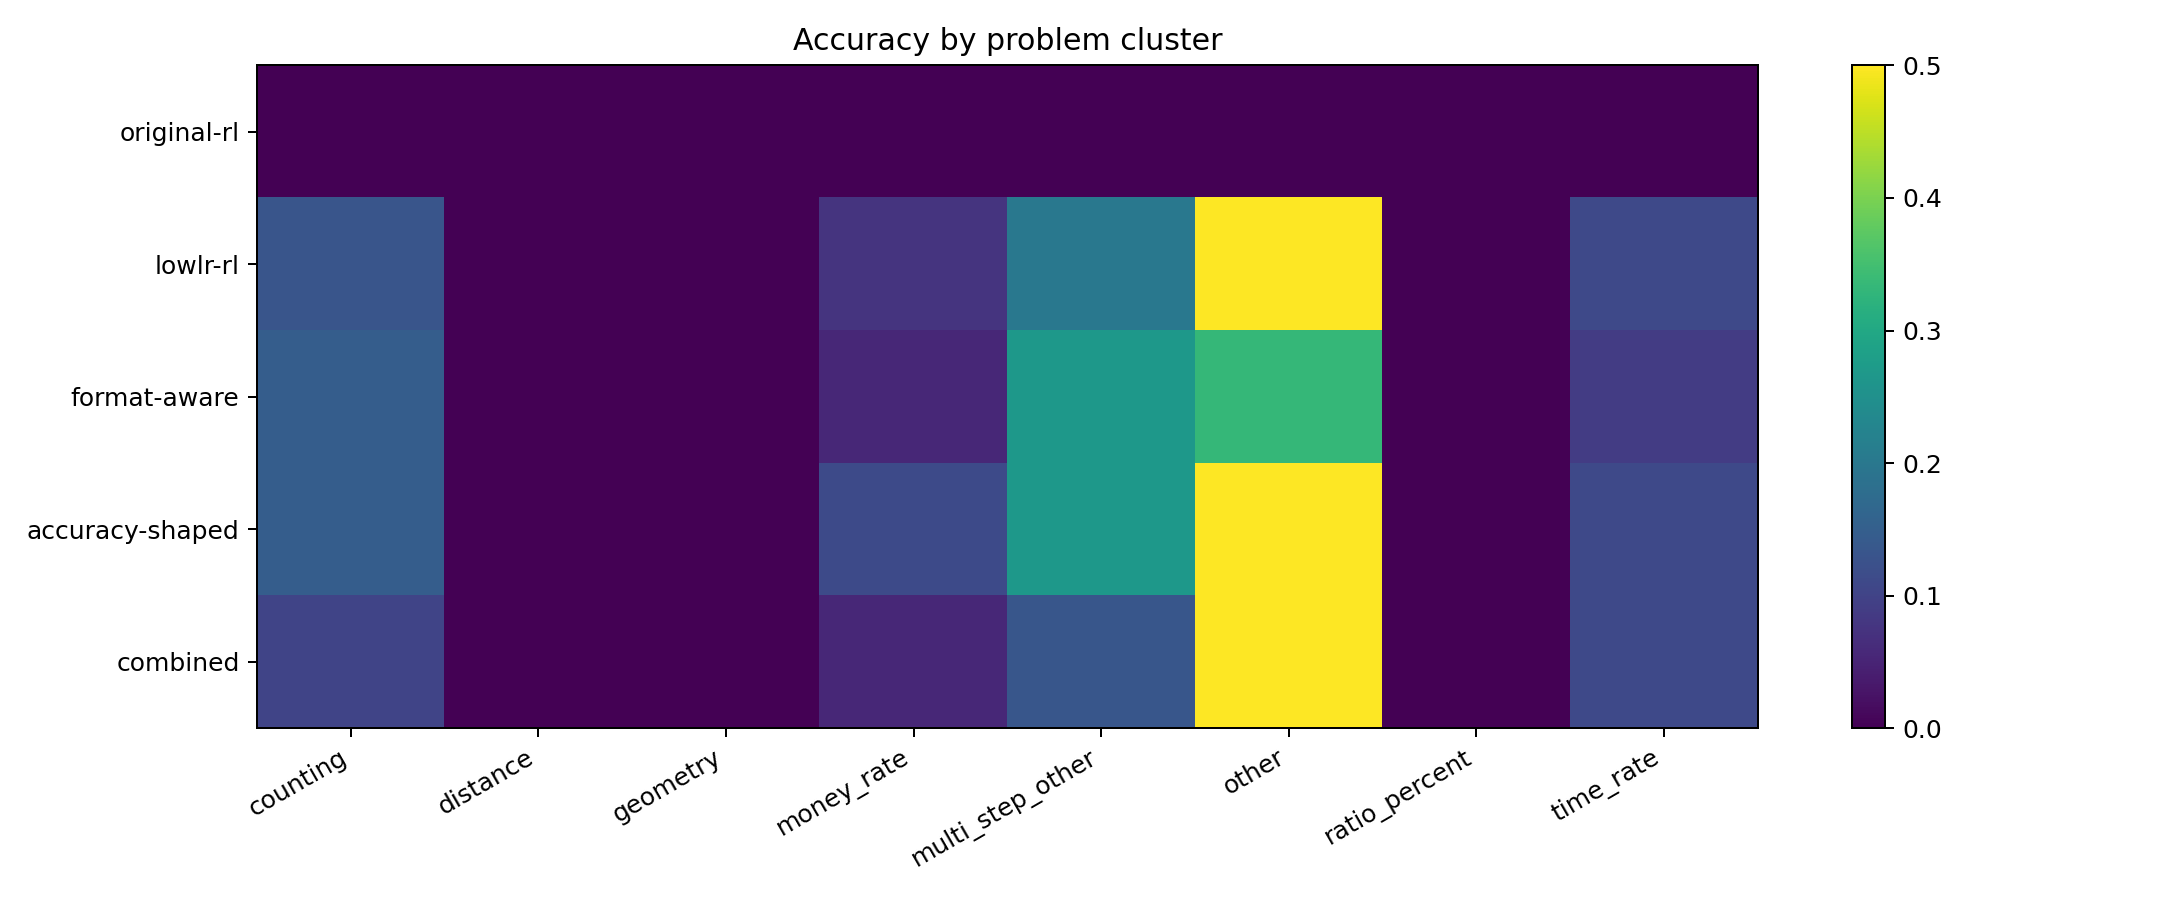
\includegraphics[width=\textwidth]{./images/section4_problem_cluster_heatmap.png}
\end{minipage}\hfill
\begin{minipage}{1.0\textwidth}
    \centering
    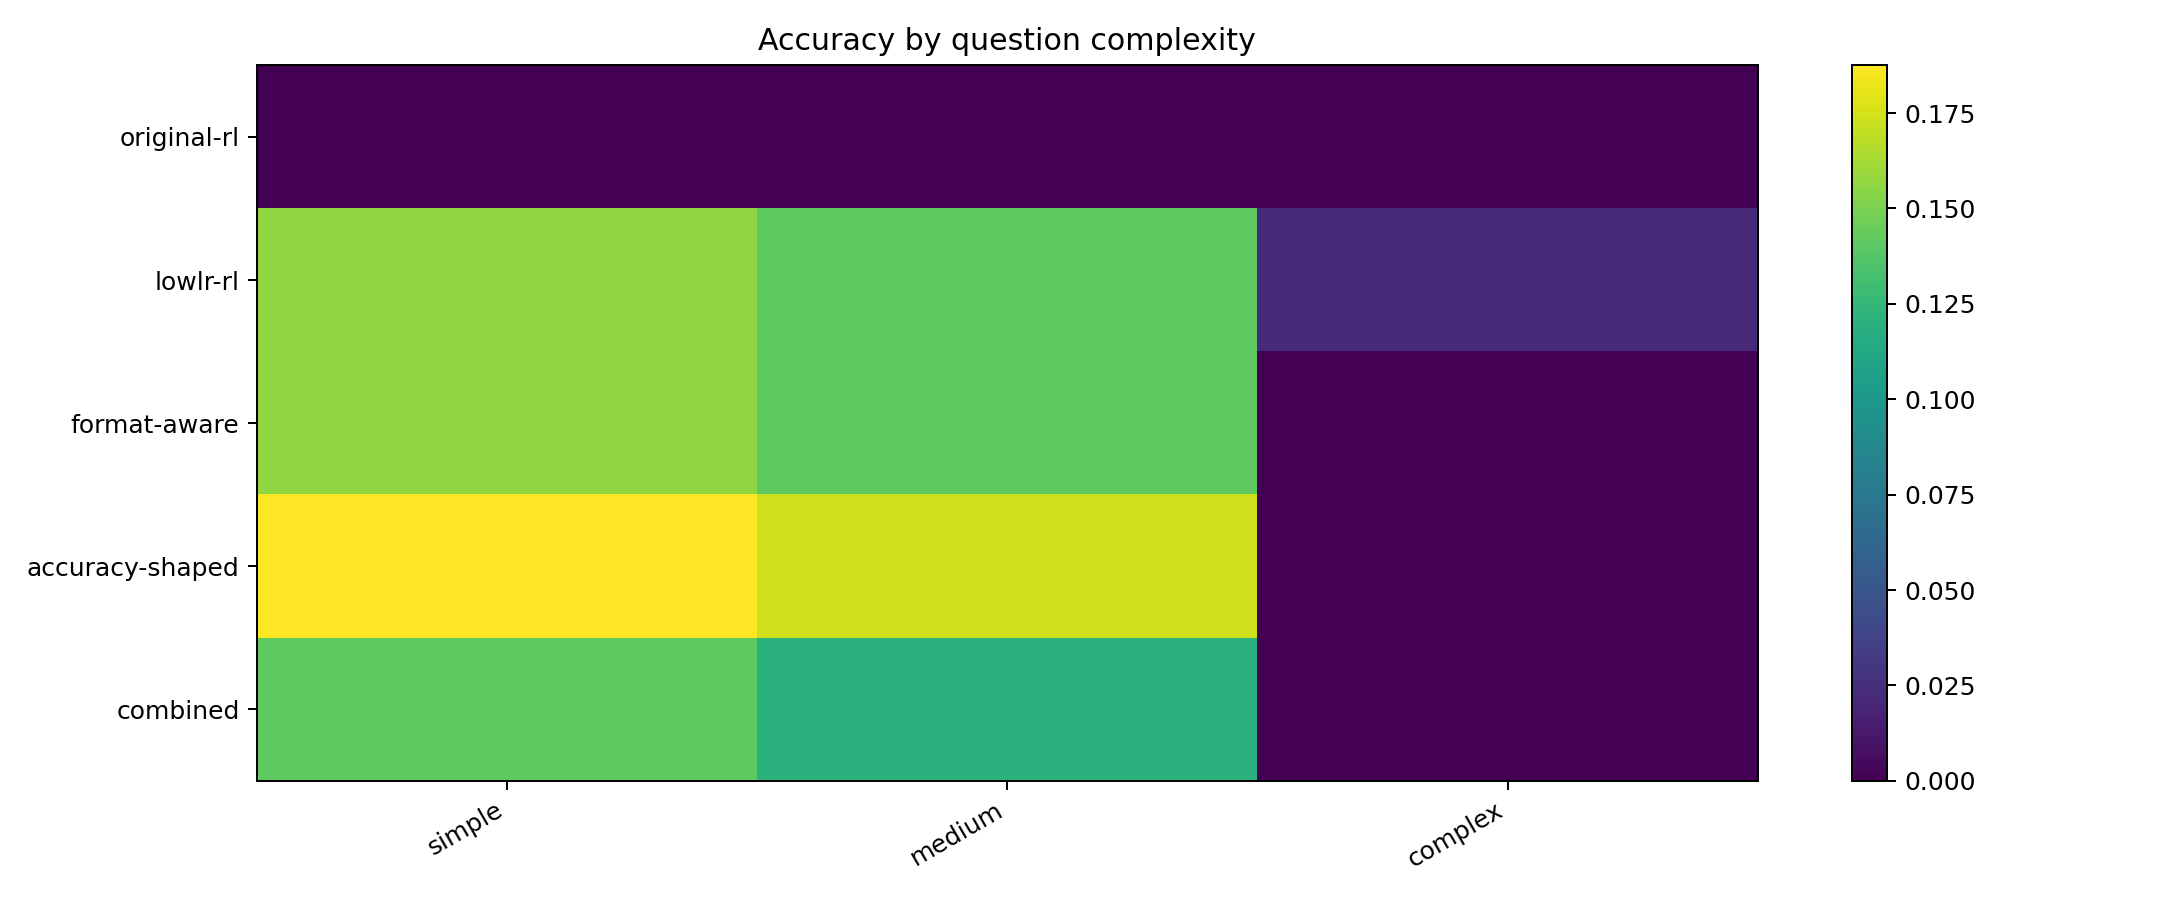
\includegraphics[width=\textwidth]{./images/section4_complexity_heatmap.png}
\end{minipage}
\caption{Accuracy by problem cluster and by question complexity. Reward shaping improves several clusters substantially over the original RL baseline, and the accuracy-shaped reward is strongest overall, but the low-learning-rate baseline remains competitive on the hardest questions.}
\label{fig:reward-clusters}
\end{figure}

At the problem-cluster level, the strongest gains appear in the \texttt{other}, \texttt{multi\_step\_other}, \texttt{counting}, \texttt{money\_rate}, and \texttt{time\_rate} clusters. The accuracy-shaped run performs best overall on \texttt{money\_rate} (0.1132) while tying the low-learning-rate and combined runs on \texttt{other} (0.5000) and matching the format-aware run on \texttt{multi\_step\_other} (0.2667). However, all three shaped rewards still achieve 0 on the strict \texttt{geometry}, \texttt{distance}, and \texttt{ratio\_percent} clusters in this analysis, and none improves on the low-learning-rate run's small but nonzero complex-question accuracy. This suggests that although denser rewards fix answer production and improve straightforward arithmetic reasoning, they do not yet solve the most compositionally demanding subfamilies of GSM8K.

\subsection{Impact of Each Reward Design}

The effect of each modification can now be stated fairly clearly:

\begin{itemize}
    \item \textbf{Format-aware reward.} This reward successfully addresses the dominant failure mode from Section \ref{section3}: it converts the model from one that mostly produces unusable outputs into one that usually emits a worked solution with a final answer marker. Relative to the low-learning-rate baseline, however, it mainly improves formatting consistency rather than final exact accuracy, and it remains slightly weaker overall.
    \item \textbf{Accuracy-shaped reward.} This is the strongest overall reward system. It achieves the best final accuracy, the highest fraction of correctly formatted answers, and the best performance on simple and medium questions. It is also the only reward system here that clearly improves on the stabilized low-learning-rate RL baseline in overall accuracy. The most plausible explanation is that rewarding worked-solution structure and near-miss answers gives the model denser feedback while still keeping exact correctness as the dominant signal.
    \item \textbf{Combined reward.} This reward remains much better than the original binary baseline, but it does not outperform the accuracy-shaped environment and it also underperforms the low-learning-rate baseline in final accuracy. The likely reason is that, with multiple partial rewards active at once, credit is spread across too many objectives and exact arithmetic receives relatively less pressure than in the accuracy-shaped design. In effect, the combined reward preserves answer structure but does not convert that structure into as many correct final answers.
\end{itemize}

Overall, these experiments lead to four main conclusions. First, we created three additional RL environments that changed only the reward system while keeping the rest of the RL setup fixed. Second, all three new rewards improved materially over the original RL run. Third, comparing against the stabilized low-learning-rate baseline shows that the accuracy-shaped reward is the only one that clearly improves on a non-collapsed RL reference, while the format-aware and combined rewards mainly improve answer structure and formatting. Fourth, the error-analysis and clustering results show that the main effect of the additional rewards is to transform failures from ``does not produce a usable answer'' into ``produces a usable but often numerically wrong answer,'' with the accuracy-shaped reward giving the best end-to-end tradeoff. This in turn suggests that the next stage of improvement should focus less on answer formatting and more on arithmetic fidelity and hard-cluster generalization.\\

The code used to conduct our experiments can be found at the URL listed below:\\ \bluehref{https://github.com/merrickliu888/nanochat/tree/a4/assignments/a4}{https://github.com/merrickliu888/nanochat/tree/a4/assignments/a4}

\begin{thebibliography}{9}
\bibitem{deepseekmath} Shao, Z., et al. (2024). DeepSeekMath: Pushing the Limits of Mathematical Reasoning in Open Language Models. arXiv preprint arXiv:2402.03300.
\bibitem{nanochat-discussion}
Karpathy, A. (2025). Nanochat Discussion \#1: Introducing nanochat: The best ChatGPT that \$100 can buy. GitHub Discussions. Available at: \url{https://github.com/karpathy/nanochat/discussions/1} (accessed March 11, 2026).

\end{thebibliography}
\end{document}
